%%%%(c)
%%%%(c)  This file is a portion of the source for the textbook
%%%%(c)
%%%%(c)    Abstract Algebra: Theory and Applications
%%%%(c)    Copyright 1997 by Thomas W. Judson
%%%%(c)
%%%%(c)  See the file COPYING.txt for copying conditions
%%%%(c)
%%%%(c)
\chap{Isomorphisms of Groups\quad
\sectionvideohref{JmyIIeUEoAU&index=30&list=PL2uooHqQ6T7PW5na4EX8rQX2WvBBdM8Qo}}{isomorph}

Thanks to Tom Judson for providing the foundational material for this chapter.

\section{Preliminary examples}
\label{sec:isomorph_defn_ex}

Several times in the book so far we have run into the idea of  \emph{isomorphic groups}\index{Group!isomorphic}.  For instance:

\begin{example}{chap1_ex}
In Chapter \ref{complex} we pointed out that ${\mathbb C}$ under complex addition and ${\mathbb R} \times {\mathbb R}$ under pairwise addition act exactly the same. In order to introduce the new concepts of this chapter, let's go over this again. 

If $z = a+bi$ and $w = c+di$ are complex numbers, we can identify  them as real ordered pairs according to the following ``translation'' function $f:\mathbb{C} \rightarrow \mathbb{R} \times \mathbb{R}$:
\[f(a+bi) = (a,b),\]
which we may also represent as
\[ a+bi \xrightarrow{f} (a,b). \]
If we add two complex numbers and ``translate'' the result to an ordered pair, we find:
\[
z + w = (a + bi) + (c + di)  \xrightarrow{f} (a+b,c+d).
\]
On the other hand, if we map $z$ and $w$ separately we get:
\[
z = a + bi  \xrightarrow{f} (a,b);\qquad w = c+di  \xrightarrow{f} (c,d),
\]
and then if we add the resulting  coordinate pairs, we obtain
\begin{align*}
(a,b) +  (c,d) 
&= (a+c,b+d). 
\end{align*}
which is the same as before. So we get the same result whether we add the complex numbers or their corresponding ordered pairs.  

What we've shown  is illustrated in Figure~\ref{fig:groups:CommDiag}. If we start with the complex numbers $z,w$, we get the same result whether we follow first the arrow to the right (``translation'' to ${\mathbb R} \times {\mathbb R}$) and then go down (addition in ${\mathbb R} \times {\mathbb R}$), or whether we follow first the down arrow (addition in ${\mathbb C}$) and then go right (``translation'' to ${\mathbb R} \times {\mathbb R}$).
%The ``translation map'' we are using is the function 
%\begin{center}
%$f : {\mathbb C} \longrightarrow {\mathbb R} \times {\mathbb R}$ such that $f(a + bi) = (a,b)$.
%\end{center}

\begin{figure}[htb]
	   \center{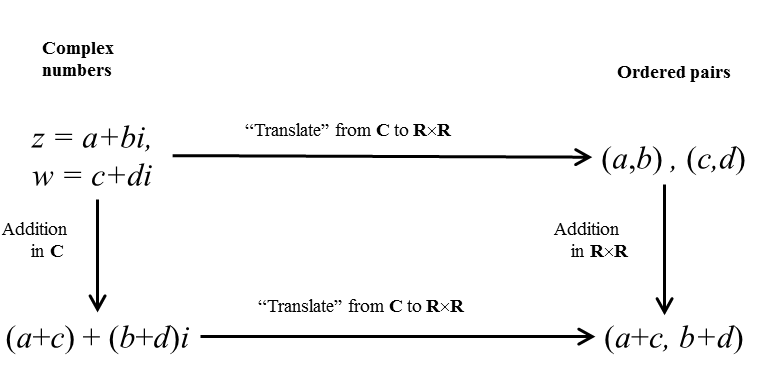
\includegraphics[width=4.in]
	         {images/CommDiag.png}}
	  \caption{\label{fig:groups:CommDiag} Addition is the ``same'' for complex numbers and real ordered pairs. }
\end{figure}

\end{example}

\begin{rem}
Readers with an eidetic memory may recognize the similarity between Figure~\ref{fig:groups:CommDiag} and Figure~\ref{fig:commDiagModular}. In fact, this type of diagram pops up a lot in higher mathematics, so much so that it has a special name: \term{commutative diagram}.
\end{rem}

\begin{exercise}{iso_1}
Let $f$ be  the function used in Example \ref{example:isomorph:chap1_ex} to rename complex numbers as ordered pairs. Recall that $r \cis \theta$ is the polar form of a complex number. How would you write $f(r \cis \theta$)?
\end{exercise}

Previously when we talked informally about two groups being isomorphic, we emphasized that  the two groups are "equivalent"  in some sense.  So for instance, in the case of Example 1 it should be possible to exchange the roles of  ${\mathbb C}$ and ${\mathbb R} \times {\mathbb R}$ and get the same result.  For this to work, there should  be a function from ${\mathbb R} \times {\mathbb R}$ to ${\mathbb C}$  that shows how to replace ordered pairs with complex numbers without ``changing anything".  What would that function be?  A prime suspect is the inverse of $f$---assuming, that is, that $f$ actually has an inverse.  What type of function does $f$ have to be in order to have an inverse?  You guessed it--a bijection.

\begin{exercise}{iso_2}
Prove that the function $f$ defined in Example~\ref{example:isomorph:chap1_ex}  is a bijection.
\end{exercise}

\begin{exercise}{iso_3} 
Draw a diagram similar to Figure~\ref{fig:groups:CommDiag}  for the function $g: {\mathbb C} \rightarrow {\mathbb R} \times {\mathbb R}$ defined by $g(a + bi) = (3a, 3b)$. Show that the same ``arrow-following'' property holds: that is, you can follow the arrows from the upper left to lower right in either order, and still end up with the same result.
\end{exercise} 

\begin{exercise}{iso_4}
Prove that the function $h(a + bi) = (a+2, b+2)$ is {\bf not} an isomorphism from ${\mathbb C}$ to  ${\mathbb R} \times {\mathbb R}$.
\hyperref[sec:isomorph:hints]{(*Hint*)}
 \end{exercise}


%With that in mind, we have a couple of questions.  Could  ${\mathbb C}$ be isomorphic to ${\mathbb Z} \times {\mathbb Z}$?  No.  Certainly it works right to left:  if we replace any two integer-ordered pairs with their corresponding complex numbers, the sum would be equivalent both ways.  But it does not work left to right.  There are complex numbers, such as $2+1.5i$, that have no integer equivalent; another way of saying this is to say that there are more complex numbers than their are integer-ordered pairs (even though the cardinality of both sets is infinity).  So there would be some complex numbers that we couldn't 

%possible footnote about countably infinite and uncountably infinite here


\begin{example}{sym_ex}
In the Symmetries chapter we also saw some  examples of isomorphic groups.  In particular, we saw that ${\mathbb Z_4}$, the $4^{th}$ roots of unity, and the rotations of a square act exactly the same under modular addition, modular multiplication, and function composition respectively. Let's remind ourselves why. 
The following are the Cayley tables for ${\mathbb Z_4}$, the $4^{th}$ roots of unity (which we'll denote by $\langle i \rangle$), and the rotations of a square ($R_4$):

\begin{table}[H]
\caption{Cayley table for ${\mathbb Z}_4$}
\label{Z4_add_table}
{\small
\begin{center}
\begin{tabular}{c|cccccccc}
$\oplus$ & 0 & 1 & 2 & 3  \\
\hline
0        & 0 & 1 & 2 & 3  \\
1       & 1 & 2 & 3 & 0  \\
2       & 2 & 3 & 0 & 1 \\
3       & 3 & 0 & 1 & 2 \\

\end{tabular}
\end{center}
}
\end{table}

\begin{table}[H]
\caption{Cayley table for $\langle i \rangle$}
\label{4_roots_table}
{\small
\begin{center}
\begin{tabular}{c|cccccccc}
$\cdot$ & 1 &$i$ & -1 & $-i$  \\
\hline
1        & 1 &$i$ & -1 &$-i$  \\
i       &$i$ & -1 & $-i$ & 1  \\
-1       & -1 & $-i$ & 1 & $i$ \\
-i       & $-i$ & 1 & $i$ & -1 \\

\end{tabular}
\end{center}
}
\end{table}

\begin{table}[H]
\caption{Cayley table for $R_4$}
\label{4_rotations_table}
{\small
\begin{center}
\begin{tabular}{c|cccccccc}
$\circ$ & $\var{id}$ & $r_{90}$ & $r_{180}$ & $r_{270}$  \\
\hline
$\var{id}$        & $\var{id}$ & $r_{90}$ & $r_{180}$ & $r_{270}$  \\
$r_{90}$       & $r_{90}$ & $r_{180}$ & $r_{270}$ & $\var{id}$  \\
$r_{180}$       & $r_{180}$ & $r_{270}$ & $\var{id}$ & $r_{90}$ \\
$r_{270}$       & $r_{270}$ & $\var{id}$ & $r_{90}$ & $r_{180}$ \\

\end{tabular}
\end{center}
}
\end{table}

\begin{enumerate}[(1)]
\item
Comparing ${\mathbb Z_4}$ and $\langle i \rangle$, notice that if we take the Cayley table for ${\mathbb Z_4}$ and make the folllowing replacements: 

\begin{align*}
  0 \rightarrow 1 \qquad
    1 \rightarrow i \qquad
    2 \rightarrow -1 \qquad
    3 \rightarrow -i, 
\end{align*}
    
then the result exactly matches the Cayley table for $\langle i \rangle$.  This means that if you add any two elements in ${\mathbb Z_4}$ (say 1 and 2), and also multiply their corresponding elements in $\langle i \rangle$ ($i$ and -1), your results from each of these actions are corresponding elements (3 and $-i$).


Hence the function $f: {\mathbb Z_4} \longrightarrow \langle i \rangle$  that takes 
\begin{align*}
    0 \xrightarrow{f} 1 ,~~     1 \xrightarrow{f} i,~~    2 \xrightarrow{f} -1,~~   3 \xrightarrow{f} -i  
\end{align*}
 is an isomorphism from ${\mathbb Z_4}$ to the $4^{th}$ roots of unity, and these groups are isomorphic to each other.

\item
Now if we compare $\langle i \rangle$ and $R_4$, using the function  $g: \langle i \rangle \longrightarrow R_4$  defined by
\begin{align*}
1 \xrightarrow{g} \var{id}, ~~\
i \xrightarrow{g}  r_{90},~~
-1 \xrightarrow{g} r_{180},~~
 -i \xrightarrow{g} r_{270}, 
\end{align*}
we see that their Cayley tables are in fact exactly the same.  Hence the $4^{th}$ roots of unity and the rotations of a square are isomorphic to each other, and $g$ is an isomorphism between them.  

\item
Finally, using the  function
$h: {\mathbb Z_4} \longrightarrow R_4$  that takes
\begin{align*}
 0\xrightarrow{h} \var{id},~~
    1 \xrightarrow{h} r_{90},~~
    2 \xrightarrow{h} r_{180},~~
    3 \xrightarrow{h} r_{270}, 
\end{align*}
we see that the Cayley tables for ${\mathbb Z_4}$ and $R_4$ are exactly the same.  Hence ${\mathbb Z_4}$ and the rotations of a square are isomorphic to each other, and $h$ is an isomorphism between them.
\end{enumerate}

\noindent
So ${\mathbb Z_4}$, $R_4$, and $\langle i \rangle$ are all isomorphic to each other. Mathematically we state this as follows:

\[ {\mathbb Z_4} \cong  R_4 \cong \langle i \rangle \]
 
 \end{example}
 
% \begin{exercise}{iso_5}
 %Prove that  the functions $f,g,h$ in Example~\ref{example:isomorph:sym_ex} are all bijections.
 %\end{exercise}
 

 \begin{exercise}{iso_7}
 Determine whether each of the following functions are isomorphisms between the groups in Example~\ref{example:isomorph:sym_ex}. Justify your answers. 
 \begin{enumerate}[(a)]
 \item
 $ f: {\mathbb Z_4}  \longrightarrow \langle i \rangle$ defined by 
\[  
f(0) = 1,~~
 f(1) = -1,~~
 f(2) = i,~~
 f(3) = -i.
\]
 
 \item
$ g: {\mathbb Z_4}  \longrightarrow R_4$ defined by 
\[ 
g(0) = {\var id},~~
 g(1) = r_{270},~~
 g(2) = r_{90} ,~~
 g(3) = r_{180}. 
 \]
 
 \item
 $ h: R_4 \longrightarrow \langle i \rangle$ defined by 
\[ 
 h(1) = {\var id},~~ 
h(i) = r_{270},~~
h(-1) = r_{180},~~
 h(-i) = r_{90}.
\]


 \item
 $ h: R_4 \longrightarrow \langle i \rangle$ defined by 
\[ 
 h({\var id}) = 1,~~ 
h(r_{270}) = i,~~
h(r_{180}) = -i,~~
 h(r_{90}) =-1.
\]

\end{enumerate}
 \end{exercise}

 \begin{exercise}{iso_6}
 Come up with a \emph{different} isomorphism for each pairing of groups in Example \ref{example:isomorph:sym_ex}. For instance, find a  function  different from $f$ that maps ${\mathbb Z_4} \longrightarrow \langle i \rangle$  that matches the the two Cayley tables. Do the same thing with $g$ and $h$.
 \end{exercise}
  
\section{Formal definition and basic properties of isomorphisms}
\label{sec:FormalDefinitionIsomorphism}

So let's buckle down and get mathematical. We start with a rigorous definition of isomorphism:

\begin{defn}\label{isomorph_defn}
Two groups $(G, \cdot)$ and $(H, \circ)$ are \term{isomorphic}\index{Group!isomorphic} if there exists a bijection $\phi : G \rightarrow H$ such that the group operation is preserved;  that~is, 
\[
\phi( a \cdot b) = \phi( a) \circ \phi( b)
\]
for all $a$ and $b$ in $G$. If $G$ is isomorphic to $H$, we write $G \cong H$. The function $\phi$ is called an \term{isomorphism}\index{Group!isomorphism of}\index{Isomorphism!of groups}. 
\end{defn}

\begin{rem}
We'll often use Greek letters ($\phi$ (`phi'), $\gamma$ ('gamma'), $\psi$('psi'), etc.) to denote isomorphisms--partially because `phi' is reminiscent of isomor$\,$`phi'$\,$sm, and partially because we don't want to confuse isomorphisms with group elements  (which are denoted by $g,h,$ and so on.)
\end{rem}

\begin{rem}
Definition~\ref{isomorph_defn} specifies that any isomorphism must be a bijection, i.e. a function that is 1-1 and onto.  Proposition~\ref{proposition:functions:InverseBijection} tells us that any function that has an inverse is a bijection, and vice versa. You'll find that often the easiest way to show that a function is a bijection is to show it has an inverse.   
\end{rem}


\begin{exercise}{iso_8}
\begin{enumerate}[(a)]
\item
Let consider the function $\phi : \mathbb{R} \rightarrow \mathbb{R}$ defined by:  $\phi(x) = 5x$.  Use Definition~\ref{isomorph_defn} to show that $\phi$ defines an isomorphism. What are the two isomorphic groups involved?
\item
Let $a$ be a nonzero real number, and consider the function $\phi_a : \mathbb{R} \rightarrow \mathbb{R}$ defined by:  $\phi_a(x) = ax$.  Show that $\phi_a$ defines an isomorphism. What are the two isomorphic groups involved?
\end{enumerate}
\end{exercise}

Some important properties of isomorphisms follow directly from the above definition. First we have:

\begin{prop}{IsoId}
Given that  $\phi : G \rightarrow H$ is an  isomorphism, then $\phi$ takes the identity to the identity: that is, if $e$ is the identity of $G$, then  $\phi(e)$ is the identity of $H$ (see Figure \ref{fig:isomorph:isomId}).
\end{prop}


\begin{figure}[htb]
	   \center{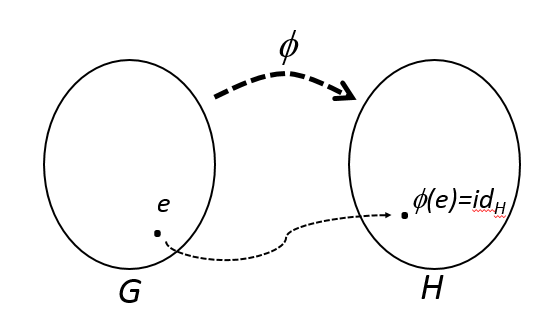
\includegraphics[width=3.5in]
	         {images/isomId.png}}
	  \caption{\label{fig:isomorph:isomId} Isomorphic image of   inverse elements are  inverse elements. }
\end{figure}


\begin{exercise}{phi_id}
Fill in the blanks in the following proof of Proposition~\ref{proposition:isomorph:IsoId}:
\medskip

\noindent
Given that $e$ is the identity of \underline{$~<1>~$} and $h$ is an arbitrary element of \underline{$~<2>~$}.  Since $\phi$ is a bijection, then there exists $g \in \underline{~<3>~}$ such that $\phi(\underline{~<4>~}) = h$.  Then  we have:
\begin{align*}
\phi(e) \circ h &= \phi(e) \circ \phi(\underline{~<5>~}) & \textrm{(substitution)}\\
&= \phi( e \cdot \underline{~<6>~}) & \textrm{(definition of~} \underline{~<7>~})\\
&= \phi( \underline{~<8>~}) & \textrm{(definition of~} \underline{~<9>~})\\
&= h & \textrm{(substitution)}
\end{align*}
Following the same steps, we can also show
\begin{align*}
h \circ \phi(e) = \underline{~<10>~}.
\end{align*}
It follows from the definition of identity that $\underline{~<11>~}$ is the identity of the group $\underline{~<12>~}$.
\end{exercise}


Another important property of isomorphisms is illustrated in Figure~\ref{fig:isomorph:isomInv}, and stated in Proposition~\ref{proposition:isomorph:IsoInv}:

\begin{figure}[htb]
	   \center{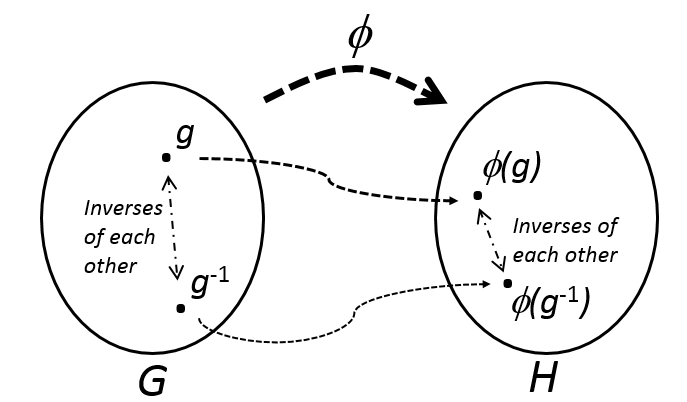
\includegraphics[width=3.5in]
	         {images/isomInv.png}}
	  \caption{\label{fig:isomorph:isomInv} Isomorphic image of an  identity element is an identity element. }
\end{figure}

\begin{prop}{IsoInv}
Given that  $\phi : G \rightarrow H$ is an  isomorphism, then $\phi$ preserves the operation of inverse: that is, for any $g \in G$ we have
\begin{equation*}
\phi(g^{-1}) = (\phi(g))^{-1}.
\end{equation*}
\end{prop}

\begin{exercise}{phi_inverse}
Fill in the blanks in the following proof of Proposition~\ref{proposition:isomorph:IsoInv}:
\medskip

\noindent
Let $e$ and $f$ be the identities of $G$ and $H$, respectively. Given that $g \in \underline{~<1>~}$, we have:
\begin{align*}
\phi(g) \circ \phi(g^{-1}) &= \phi(g \cdot g^{-1}) & \textrm{(definition of}~\underline{~<2>~})\\
&= \phi(e) &\textrm{(definition of}~\underline{~<3>~})\\
&= f &\textrm{(Proposition}~\underline{~<4>~} ).
\end{align*}
Using the same steps, we can also show
\begin{align*}
\phi(g^{-1}) \circ \phi(g) = \underline{~<5>~}.
\end{align*}
By the definition of inverse, it follows that
\begin{align*}
( \phi(g))^{-1} = \underline{~<6>~}.
\end{align*}
\end{exercise} 

It's possible to use isomorphisms to create other isomorphisms:

\begin{exercise}{InvCompIso}
\begin{enumerate}[(a)]
\item
Given that  $\phi : G \rightarrow H$ is an  isomorphism, show that  $\phi^{-1} : H \rightarrow G$ is also an  isomorphism.
\hyperref[sec:isomorph:hints]{(*Hint*)}
\item
Given that  $\phi : G \rightarrow H$ and $\psi : H \rightarrow K$ are  isomorphisms, show that  $\psi \circ\phi:G \rightarrow K$ is also an  isomorphism.
\hyperref[sec:isomorph:hints]{(*Hint*)}
\end{enumerate}
\end{exercise}

We said in the previous section that isomorphic groups are ``equivalent'' in some sense. This fact has a formal mathematical statement as well:

\begin{prop}{GpEquivRel}
Isomorphism is an equivalence relation on groups. 
\end{prop}

\begin{exercise}{GpEquivRel}
Prove Proposition~\ref{proposition:isomorph:GpEquivRel}.
\hyperref[sec:isomorph:hints]{(*Hint*)}
\end{exercise}

\section{Examples and generalizations}
\label{sec:iso_more_ex}

\subsection{Examples of isomorphisms}
Now that we have a formal definition of what it means for two groups to be isomorphic, let's look at some more examples, in order to get a good feel for identifying groups that are isomorphic and those that aren't.
%In the previous examples we only looked at isomorphisms between finite groups.  This simplified our proof process in a couple ways.  One, in showing that the isomorphism was a bijection, all we had to do was verify it visually with the arrow diagram we created, because the arrow diagram contained all the information needed to show that the function was one-to-one and onto.  Two, to show that the function preserved the operations of the respective groups, all we needed was to verify it visually with the Cayley tables, since again the Cayley tables contained all the information needed.

%We were able to take advantage of visual tools like these because the groups we were dealing with were finite (and relatively small in number), and therefore we could represent all the information we needed concisely in a "picture".  However, if we were proving that two \emph{infinite} groups were isomorphic, it would be physically impossible to construct the required arrow diagrams or Cayley tables.  For that matter, if the two groups were finite but large in number, though you could construct the arrow diagrams and Cayley tables, the time required for such an endeavor would make the proof process very long.

%So in such cases, it is necessary to prove our two properties of isomorphisms--that they are bijections and that they preserve the group operations--using the functional and algebraic proofs we introduced in Chapters 4 and 9.  For instance:

From high school and college algebra we are well familiar with the fact that when you multiply exponentials (with the same bases), the result of this operation is the same as if you had just kept the base and added the exponents.  This equivalence of operations is a telltale sign for identifying possible isomorphic groups.  The next two examples illustrate this observation.

For our first example, we   denote the set of integer powers of 2 as $2^{\mathbb Z}$, that is:
\[ 2^{\mathbb Z} \equiv \{\ldots, 2^{-2}, 2^{-1}, 2^0, 2^1, 2^2, \ldots\}. \]
\begin{exercise}{}
Show that $2^{\mathbb Z}$ with the operation of multiplication is a subgroup of ${\mathbb Q}^{\ast}$.
\end{exercise}

\begin{example}{rational_isomorph}
When elements of $2^{\mathbb Z}$ are multiplied together, their exponents add: we know this from basic algebra. This suggests there should be an isomorphism between ${\mathbb Z}$ and   $2^{\mathbb Z}$. In fact, we may define the function
$\phi: {\mathbb Z} \rightarrow 2^{\mathbb Z}$ by $\phi( n ) = 2^n$.
To show that this is indeed an isomorphism, by our definition we must show two things: (a)  that the function preserves the operations of the respective groups; and (b) that the function is a bijection:
\begin{enumerate}[(a)] 
\item
We may compute
\[
\phi( m + n ) = 2^{m + n} = 2^m 2^n = \phi( m ) \phi( n ).
\]
\item
By definition the function $\phi$ is onto the subset $\{2^n :n \in {\mathbb Z} \}$ of  ${\mathbb Q}^\ast$.  To show that the map is injective, assume that $m \neq n$.  If we can show that $\phi(m) \neq \phi(n)$, then we are done.  Suppose that $m>n$ and assume that $\phi(m) = \phi(n)$.  Then $2^m = 2^n$ or $2^{m-n} = 1$, which is impossible since $m-n>0$. 
\end{enumerate}

This completes the proof that $ {\mathbb Z} \cong 2^{\mathbb Z}$.
\end{example}      

 
\begin{example}{RealIsomorph}
As in the previous example, the real powers of $e$ under multiplication acts exactly like addition of those real exponents.  
This suggests that the function $\psi(x)=e^x$ is an isomorphism between an additive group and a multiplicative group.  The reader will complete this proof of this fact as an exercise.  
\end{example}

\begin{exercise}{e_isomorph_proof}
Define the function $\psi$ by: $\psi(x) = e^x$ for $x \in \mathbb{R}$.
\begin{enumerate}[(a)]
\item
Given that the domain of $\psi$ is all real numbers, what is the range of $\psi$?
\item
Prove that $\psi(x)$ is a bijection between its domain and range.
\item
Find group operations on the domain and range of $\psi$ such that $\psi(x)$ preserves operations; i.e. $\psi(x \cdot y) = \psi(x)\compose \psi(y)$, where $\cdot$  and $\compose$ are the group operations on the domain and range,respectively. Verify that $\psi$ does indeed preserve operations for these two operations.
\item
Now that we know $\psi(x)$ is an isomorphism, what can we conclude about $({\mathbb R}^+,\cdot)$ and $({\mathbb R},+)$?
\end{enumerate}
\end{exercise}

\begin{exercise}{ln_isomorph_proof}
\begin{enumerate}[(a)]
\item
What is the largest possible domain and range of the natural logarithm function $\ln(x)$? (Consider only real logarithms,and not complex-valued logarithms or logarithms of complex numbers.)
\item
Using the previous exercise, the relation between natural logarithm and exponential function, as well as a result from earlier in this chapter, show that the natural logarithm function is an isomorphism. What are the two isomorphic groups?
\item
Using the fact that $\log_{10}(x) = \ln(x) / \ln(10)$, show that the base 10 logarithm function is also an isomorphism.  What are the two isomorphic groups?
\item 
Given any two positive real numbers ($a$ and $b$)  in scientific notation that are accurate to 3 decimal places, show how you may estimate $ab$ using addition and a table containing the base 10 logarithms of all integers from 100 to 999.  For example, how would you compute the product $(1.75 \times 10^{15})(9.53 \times 10^{-27}$?
\end{enumerate}
\end{exercise}

\begin{exercise}{iso_prac1}
Prove that ${\mathbb Z} \cong n{\mathbb Z}$,  for every nonzero integer $n$.
\end{exercise}
 
\begin{exercise}{iso_prac2}
Prove that ${\mathbb C}^\ast$ is isomorphic to the subgroup of $GL_2(
{\mathbb R} )$ consisting of all  matrices of the form ($a$ and $b$ are real numbers)
\[
\begin{pmatrix}
a & b \\
-b & a
\end{pmatrix}
\], where $a^2 + b^2 \neq 0$.

\noindent
(In your proof, you should verify that this set of matrices is indeed a subgroup of $GL_2(
{\mathbb R} )$: in other words, check that the determinant is never zero, when $a^2 + b^2 \neq 0$.)
\end{exercise}


\begin{example}{nonisom}
Consider the groups ${\mathbb Z}_8$ and ${\mathbb Z}_{12}$. Can you tell right away that there can't be an isomorphism between them?  Remember, an isomorphism is a one-to-one and onto function: but since 
$|{\mathbb Z}_{12}|>|{\mathbb Z}_{8}|$ there is no onto function from ${\mathbb Z}_8$ to ${\mathbb Z}_{12}$, and so they can't be isomorphic to each other.  Similarly it can be shown that any two finite groups that have differing numbers of elements can't be isomorphic to each other.
\end{example}

Let's look at some more examples where Cayley tables can help determine isomorphism.

\begin{example}{Cayley_noniso}
The following are the Cayley tables for ${\mathbb Z}_4$ and $U(5)$.

\begin{table}[H]
\caption{Cayley table for ${\mathbb Z}_4$}
\label{Z4_add_table}
{\small
\begin{center}
\begin{tabular}{c|cccccccc}
$\oplus$ & 0 & 1 & 2 & 3  \\
\hline
0        & 0 & 1 & 2 & 3  \\
1       & 1 & 2 & 3 & 0  \\
2       & 2 & 3 & 0 & 1 \\
3       & 3 & 0 & 1 & 2 \\

\end{tabular}
\end{center}
}
\end{table}

\begin{table}[H]
\caption{Cayley table for $U(5)$\label{U5_table}}
{\small
\begin{center}
\begin{tabular}{c|cccccccc}
$\odot$ & 1 & 2 & 3 & 4  \\
\hline
1        & 1 & 2 & 3 & 4  \\
2       & 2 & 4 & 1 & 3  \\
3       & 3 & 1 & 4 & 2 \\
4       & 4 & 3 & 2 & 1 \\

\end{tabular}
\end{center}
}
\end{table}

Notice that the main diagonals (left to right) of the Cayley tables seem to have a different pattern.  The main diagonal for ${\mathbb Z}_4$ is the alternating sequence, $0, 2, 0, 2$, while the main diagonal of $U(5)$ is the  non-alternating sequence $1, 4, 4, 1$.  It appears at first sight that these two groups must be non-isomorphic.  However, we may rearrange the row and column labels  in Table~\ref{U5_table} to obtain Table~\ref{U5_table2}. From the rearranged table we may read off the isomorphism: $0 \rightarrow 1, 1\rightarrow 2, 2\rightarrow 4, 3 \rightarrow 3$.

\begin{table}[H]
\caption{Rearranged Cayley table for $U(5)$\label{U5_table2}}

{\small
\begin{center}
\begin{tabular}{c|cccccccc}
$\odot$ & 1 & 2 & 4 & 3  \\
\hline
1        & 1 & 2 & 4 & 3  \\
2       & 2 & 4 & 3 & 1  \\
4       & 4 & 3 & 1 & 2 \\
3       & 3 & 1 & 2 & 4 \\

\end{tabular}
\end{center}
}
\end{table}

Note the important point that when we rearranged the table, we used the \emph{same} ordering $(1,2,4,3)$ for both rows and columns.   You don't want to use one ordering for rows, and a different ordering for columns.
\end{example} 

\begin{example}{units}
Consider  the group of units of ${\mathbb Z}_8$ and the group of units of ${\mathbb Z}_{12}$; i.e. $U(8)$ and $U(12)$.  We've seen that these  consist of the elements in ${\mathbb Z}_8$ and ${\mathbb Z}_{12}$, that are relatively prime to $8$ and $12$, respectively, so

\begin{align*}
U(8) & = \{1, 3, 5, 7 \} \\
U(12) & = \{1, 5, 7, 11 \}.
\end{align*}

\begin{exercise}{U8_U12_Cayley}
Give the Cayley tables for $U(8)$ and $U(12)$.
\end{exercise}

An isomorphism $\phi : U(8) \rightarrow U(12)$ is given by
\begin{align*}
1 & \xrightarrow{\phi}  1 \\
3 & \xrightarrow{\phi}  5 \\
5 & \xrightarrow{\phi}  7 \\
7 & \xrightarrow{\phi}  11.
\end{align*}

$\phi$ is one-to-one and onto by observation, and we can verify that $\phi$ preserves the operations of $U(8)$ and $U(12)$ by showing that replacing elements in the Cayley table of $U(8)$ according to the isomorphism $\phi$ gives the Cayley table of $U(12)$ .  Hence $U(8) \cong U(12)$.
\end{example}
The function $\phi$ is not the only possible isomorphism between $U(8)$ and $U(12)$.  

\begin{exercise}{U8_U12_other}
\begin{enumerate}[(a)]
\item
Using Cayley tables, show that the function $\psi$ defines an isomorphism  between $U(8)$ and $U(12)$, where:
\begin{align*}
1 & \xrightarrow{\psi}  1 \\
3 & \xrightarrow{\psi}  7 \\
5 & \xrightarrow{\psi}  11 \\
7 & \xrightarrow{\psi}  5.
\end{align*}
(You will have to rearrange rows and columns to get the identification between tables.)
\item
Define a different isomorphism between $U(8)$ and $U(12)$, and use Cayley tables to verify that it's an isomorphism. 
\end{enumerate}
\end{exercise}

\begin{exercise}{U8_U12_Z2Z2}
Prove that both $U(8)$ and $U(12)$ are isomorphic to ${\mathbb Z}_2 \times {\mathbb Z}_2$ (recall $\mathbb{Z}_2 \times \mathbb{Z}_2$ is the set of all pairs $(a,b)$ with $a,b \in \mathbb{Z}_2$, where 
the group operation is addition mod 2 on each element in the pair). 
\end{exercise}

 \begin{exercise}{iso_prac3}
Prove that $U(8)$ is isomorphic to the group of matrices
\[
\begin{pmatrix}
1 & 0 \\
0 & 1
\end{pmatrix},
\begin{pmatrix}
1 & 0 \\
0 & -1
\end{pmatrix},
\begin{pmatrix}
-1 & 0 \\
0 & 1
\end{pmatrix},
\begin{pmatrix}
-1 & 0 \\
0 & -1
\end{pmatrix}.
\]
\end{exercise} 

\begin{exercise}{iso_prac4}
Show that the matrices
\begin{gather*}
\Big\{
\begin{pmatrix}
1 & 0 & 0 \\
0 & 1 & 0 \\
0 & 0 & 1
\end{pmatrix},
\begin{pmatrix}
1 & 0 & 0 \\
0 & 0 & 1 \\
0 & 1 & 0
\end{pmatrix},
\begin{pmatrix}
0 & 1 & 0 \\
1 & 0 & 0 \\
0 & 0 & 1
\end{pmatrix}, \\
\begin{pmatrix}
0 & 0 & 1 \\
1 & 0 & 0 \\
0 & 1 & 0
\end{pmatrix},
\begin{pmatrix}
0 & 0 & 1 \\
0 & 1 & 0 \\
1 & 0 & 0
\end{pmatrix},
\begin{pmatrix}
0 & 1 & 0 \\
0 & 0 & 1 \\
1 & 0 & 0
\end{pmatrix}
\Big\}
\end{gather*}
form a group. Find an isomorphism of $G$ with a more familiar group of
order~6.
\end{exercise} 

\begin{example}{factor_S3_iso}
In Example~\ref{example:cosets:factor_S3} of the Cosets chapter, we looked at  the normal subgroup  $N = \{ (1), (123), (132)  \}$ of $S_3$.
The cosets of $N$ in $S_3$ were $N$ and $(12) N$; and the quotient group $S_3
/ N$ had the following multiplication table.
\begin{center}
\begin{tabular}{c|cc}
         & $N$      & $(12) N$ \\
\hline
$N$      & $N$      & $(12) N$ \\
$(12) N$ & $(12) N$ & $N$
\end{tabular}
\end{center}

You may verify that  $N$ is in fact the group of all even permutations on three elements, that is $A_3$; and $(12) N = \{ (12), (13), (23) \}$ is the set of odd
permutations. The information captured in $S_3/N$ is parity; that is,
multiplying two even or two odd permutations results in an even
permutation, whereas multiplying an odd permutation by an even
permutation yields an odd permutation. This suggests a possible isomorphism to ${\mathbb Z}_2$.
\end{example}

%Let's look at an interesting example of isomorphic groups that was brought up and hinted at in the Cosets chapter %(Example~\ref{example:cosets:factor_S3}. 

\begin{exercise}{factor_S3}
Prove that the quotient group $S_3/A_3 \cong {\mathbb Z}_2$.
\end{exercise}

In Section~\ref{sec:factor_groups} of the Cosets chapter we hinted at several examples of possible isomorphisms,  which we'll have you prove now:

\begin{exercise}{factor_iso}
Prove the following:
\begin{enumerate}[(a)]
\item
 ${\mathbb Z}/ 3 {\mathbb Z} \cong {\mathbb Z}_3$
\item
$D_n / R_n \cong {\mathbb Z}_2$
\end{enumerate}
\end{exercise}

\begin{exercise}{factor_iso2}
Based on your work in Exercise~\ref{exercise:cosets:factor_cayley_prac} prove the following:
\begin{enumerate}[(a)]
\item
 ${\mathbb Z}/ 6 {\mathbb Z} \cong {\mathbb Z}_6 $

\item
 ${\mathbb Z}_{24} / \langle 8 \rangle \cong {\mathbb Z}_8 $ 

\item
$U(20) / \langle 3 \rangle \cong  {\mathbb Z}_2 $

\end{enumerate}
\end{exercise}

We've seen several examples where  Cayley tables were used to show that two groups are isomorphic. (Of course, this works best if the groups are not too large, and it certainly doesn't work if the groups are infinite!)  Let's now consider how we can use Cayley tables to show when groups are \emph{not} isomorphic to each other. Caution: it's not enough to have Cayley tables for the two groups that don't match---we saw in Example~\ref{example:isomorph:Cayley_noniso} that even when tables don't match, it may still be possible to rearrange one of the tables to create a matchup.

Suppose  that if $T$ is a Cayley table of a group $G$. Then $g \in G$  appears on the diagonal of $T$ if and only if there is an element $g' \in G$ such that $g' \cdot g' = g$.  It turns out that this property is preserved under isomorphism:

\begin{prop}{Cayleydiag2}
Given a Cayley table $T$ for a finite group $G$, and let $g \in G$  appears on the diagonal of $T$. Let $\phi:G \rightarrow H$ be an isomorphism, and let $T'$ be a Cayley table of $H$. Then $\phi(g)$ appears on the diagonal of $T'$.
\end{prop}

\begin{proof}
As stated above, $g$ appears on the diagonal of $T$ if and only if there exists $g' \in G$ such that $g' \cdot g' = g$.  Since $\phi$ is an isomorphism, this implies $\phi(g') \cdot \phi(g') = \phi(g)$, which in turn implies that $\phi(g)$ appears on the diagonal of $T'$.
\end{proof}

\begin{prop}{CayleyDiagNum2}
Given a Cayley table $T$ for a finite group $G$, and suppose the element $g \in G$ appears $m$ times on the diagonal of $T$.  Let $\phi:G \rightarrow H$ be an isomorphism, and let $T'$ be a Cayley table of $H$. Then $\phi(g)$ appears $m$ times  on the diagonal of $T'$.
\end{prop}

\begin{exercise}{CayleyDiagNumProof2}
Prove Proposition~\ref{proposition:isomorph:CayleyDiagNum2}.
\end{exercise}

\begin{prop}{CayleyDiagNum}
Given a Cayley table $T$ for a finite group $G$, and suppose $n$ distinct elements of $G$ appear on the diagonal of $T$.  Let $\phi:G \rightarrow H$ be an isomorphism, and let $T'$ be a Cayley table of $H$. Then $n$ distinct elements of $H$ appear on the diagonal of $T'$.
\end{prop}

\begin{exercise}{CayleyDiagNumProof}
Prove Proposition~\ref{proposition:isomorph:CayleyDiagNum}.
\end{exercise}


\begin{exercise}{another_pattern}
By using the preceding propositions and comparing diagonal elements of Cayley tables, prove  that ${\mathbb Z}_4 \ncong U(12)$.
\end{exercise} 

\begin{exercise}{iso_prac5}
Prove or disprove: $U(8) \cong {\mathbb Z}_4$.
\end{exercise}
  
\begin{exercise}{iso_prac6}
Let $\sigma$ be the permutation $(12)$, and let $\tau$ be the permutation $(34)$.
Let $G$ be the set $\{ \var{id}, \sigma, \tau, \sigma\tau \}$ together with the operation of composition.
\begin{enumerate}[(a)]
\item
Give the Cayley table for the group $G$.
\item
Prove or disprove: $G \cong {\mathbb Z}_4$.
\item
Prove or disprove: $G \cong U(12)$.
\end{enumerate}
\end{exercise}



%$\psi$ by $\psi(1) = 1$, $\psi(3) = 11$, $\psi(5) = 5$, $\psi(7) = 7$. In fact, both of these groups are isomorphic to 

\begin{example}{not_isomorph_abelian}
Even though $D_3$ and ${\mathbb Z}_6$ possess the same number of elements, we might suspect that they are not isomorphic, because ${\mathbb Z}_6$ is abelian and $D_3$ is non-abelian.  Let's see if the  Cayley tables can help us here:

\begin{table}[H]
{\small
\begin{center}
\begin{tabular}{c|cccccc}
$\circ$  & $\var{id}$     & $\rho_1$ & $\rho_2$ & $\mu_1$ & $\mu_2$ & $\mu_3$ \\
\hline
$\var{id}$     & $\var{id}$     & $\rho_1$ & $\rho_2$ & $\mu_1$ & $\mu_2$ & $\mu_3$ \\
$\rho_1$ & $\rho_1$ & $\rho_2$ & $\var{id}$     & $\mu_3$ & $\mu_1$ & $\mu_2$ \\
$\rho_2$ & $\rho_2$ & $\var{id}$     & $\rho_1$ & $\mu_2$ & $\mu_3$ & $\mu_1$ \\
$\mu_1$  & $\mu_1$  & $\mu_2$  & $\mu_3$  & $\var{id}$    & $\rho_1$& $\rho_2$\\
$\mu_2$  & $\mu_2$  & $\mu_3$  & $\mu_1$  & $\rho_2$& $\var{id}$    & $\rho_1$\\
$\mu_3$  & $\mu_3$  & $\mu_1$  & $\mu_2$  & $\rho_1$& $\rho_2$& $\var{id}$
\end{tabular}
\end{center}
}
\caption{Cayley table for $D_3$}
\label{D3_table}
\end{table}

\begin{table}[H]
\caption{Cayley table for ${\mathbb Z}_6$}
\label{Z6_add_table}
{\small
\begin{center}
\begin{tabular}{c|cccccccc}
$\oplus$ & 0 & 1 & 2 & 3 & 4 & 5  \\
\hline
0        & 0 & 1 & 2 & 3 & 4 & 5  \\
1       & 1 & 2 & 3 & 4 & 5 & 0  \\
2       & 2 & 3 & 4 & 5 & 0 & 1\\
3       & 3 & 4 & 5 & 0 & 1 & 2 \\
4       & 4 & 5 & 0 & 1 & 2 & 3 \\
5       & 5 & 0 & 1 & 2 & 3 & 4 \\

\end{tabular}
\end{center}
}
\end{table}

Note that the Cayley table for ${\mathbb Z}_6$ is symmetric across the main diagonal while the Cayley table for $D_3$ is not.  Furthermore, no matter how we rearrange the row and column headings for the Cayley table for ${\mathbb Z}_6$, the  table will always be symmetric. It follows that there is no way to to match up the two groups' Cayley tables: so $D_3 \ncong {\mathbb Z}_6$.

This  argument via Cayley table works in the case where the two groups being compared are both small, but if the groups are large then it's far too time-consuming (especially if the groups are infinite!). So let us take a different approach, and fall back on our time-tested strategy of proof by contradiction. In the case at hand, this means that we first suppose that $D_3 \cong {\mathbb Z}_6$, and  then find a contradiction based on that supposition. 

So, suppose that the two groups are isomorphic, which means there exists an isomorphism $\phi : {\mathbb Z}_6 \rightarrow  D_3$.  Let $a , b \in D_3$ be two elements such that $a\circ b \neq b \circ a$.  Since $\phi$ is an isomorphism, there exist elements $m$ and $n$ in ${\mathbb Z}_6$ such~that 
\[
\phi( m )  = a \quad \text{and} \quad
\phi( n )  = b.
\]
However,
\[
a\circ b = \phi(m ) \circ  \phi(n) = \phi(m \oplus  n) = \phi(n \oplus m) = \phi(n ) \circ \phi(m) = b \circ a,
\]
which contradicts the fact that $a$ and $b$ do not commute.
\end{example}

Although we have only proven the non-isomorphicity of abelian and non-abelian groups for one particular case, the same  method of proof can be used to prove the following general result.
%Notice that in the general method for proving $D_3 \ncong {\mathbb Z}_6$, the elements $a, b, m$ and $n$ used were completely general and could have been picked from any two groups, one abelian and one not.  Therefore, that proof would work just as well for proving that any abelian group couldn't be isomorphic to a non-abelian group.  Hence 

\begin{prop}{abelian_non-abelian}
If $G$ is an abelian group and $H$ is a non-abelian group, then $G \ncong H$.
\end{prop}

\begin{exercise}{}
Prove Proposition ~\ref{proposition:isomorph:abelian_non-abelian} by imitating the proof in Example ~\ref{example:isomorph:not_isomorph_abelian}.
\end{exercise}

\begin{exercise}{iso_prac7}
Prove $D_4 \ncong {\mathbb Z}_8$.
\end{exercise}

\begin{exercise}{iso_prac8}
Prove  ${\mathbb Z}/ 6 {\mathbb Z} \ncong S_3$.
\end{exercise}


Finally, let's look at ${\mathbb Z}$ and ${\mathbb R}$.  We know ${\mathbb Z}$ is a cyclic group with $1$ as the generator, while ${\mathbb R}$ is not cyclic. (Do you remember why?)  We might suspect  that  ${\mathbb Z} \ncong {\mathbb R}$, since one group is cyclic and the other isn't.  This is in fact true, and we'll prove it.   Since ${\mathbb Z}$ and ${\mathbb R}$ are infinite groups we can't use Cayley tables, so we have to use another method (three guesses as to what it is):

\begin{prop}{not_isomorph_cyclic}
${\mathbb Z}$ is not isomorphic to ${\mathbb R}$.
\end{prop}
\begin{proof}
We will use a proof by contradiction.   Suppose that there exists an isomorphism $\phi: {\mathbb Z} \rightarrow {\mathbb R}$.  Choose any $x \in {\mathbb R}$, and let $m \in {\mathbb Z}$ be the pre-image of $x$, so that $\phi(m) = x$.  It follows that: 

\begin{align*}
x &= \phi(m) = \phi(\underbrace{1 + \ldots + 1}_{m~\textrm{times}})= \underbrace{\phi(1) + \ldots + \phi(1)}_{m~\textrm{times}}.
\end{align*}
Thus $x \in \langle  \phi(1) \rangle$.  But since this is true for \emph{any} $x \in {\mathbb R}$, this means that  $\phi(1)$ is a generator of  ${\mathbb R}$, which means that ${\mathbb R}$ is cyclic. But we've already seen that 
${\mathbb R}$ is \emph{not} cyclic. This contradiction shows that our original supposition must be false: namely, there \emph{cannot} exist an isomorphism $\phi: {\mathbb Z} \rightarrow {\mathbb R}$. This completes the proof.
\end{proof}

\noindent
Again we can generalize this proof to prove that a cyclic group cannot be isomorphic to a non-cyclic group. The contrapositive of this statement is:

\begin{prop}{cyclic_noncyclic}
If $G$ is cyclic and $G \cong H$, then $H$ is also cyclic.
\end{prop}


\begin{exercise}{cyclic_noncyclic} 
Prove Proposition \ref{proposition:isomorph:cyclic_noncyclic}.
\hyperref[sec:isomorph:hints]{(*Hint*)}
\end{exercise}



\begin{exercise}{noniso_cyclic}
\begin{enumerate}[(a)]
\item
Prove that ${\mathbb Q}$ is not isomorphic to ${\mathbb Z}$.
\item
Prove that  ${\mathbb Z}_3 \times {\mathbb Z}_3$ is not isomorphic to ${\mathbb Z}_9$. 
\item
Prove that  $D_4 \ncong {\mathbb Z}_{24} / \langle 8 \rangle$
\end{enumerate}
\end{exercise}

In the foregoing examples, the reader might develop the impression that isomorphisms must be functions between two different groups. But such is not the case!  It is quite possible for a group to be isomorphic to itself.

\begin{exercise}{autoMorph}
\begin{enumerate}[(a)]
\item
Given any group $G$, let $\var{Id}:G \rightarrow G$ be the identity map, that is, $\var{Id}(g)=g$ for all $g \in G$.  show that $\var{Id}$ is an isomorphism.
\item
Let $\mathbb{M}_n(\mathbb{R})$ be the group of $n\times n$ matrices with real entries under the addition operation. Prove that the transpose function $M \rightarrow M^T$ is an isomorphism from  $\mathbb{M}_n(\mathbb{R})$ to $\mathbb{M}_n(\mathbb{R})$.
\end{enumerate}
\end{exercise}

An isomorphism from a group to itself is called an \emph{automorphism}\index{Automorphism!of a group}\index{Group!automorphism}.


\subsection{General properties of isomorphisms\quad
\sectionvideohref{AI2JXYaaV8U&index=31&list=PL2uooHqQ6T7PW5na4EX8rQX2WvBBdM8Qo}}\label{iso_properties}
In the last two sections we  proved several properties of isomorphic groups and their corresponding isomorphisms.  We collect these properties (and add a few more) in the following proposition:

\begin{prop}{isomorph_theorem_1}
Let $\phi : G \rightarrow H$ be an isomorphism of two groups.  Then the following statements are true. 
\begin{enumerate}[(1)]
 

\rm \item 
$|G| = |H|$. 

\rm \item 
$\phi^{-1} : H \rightarrow G$ is an isomorphism. 

\rm \item 
$G$ is abelian if and only if $H$ is abelian. 

\rm \item 
$G$ is cyclic if and only if $H$ is cyclic. 

\rm \item
If $g \in G$ is an element of order $n$ (that is, $| \langle g \rangle | = n$), then 
$\phi(g) \in H$ is also an element of order $n$.

\rm \item 
If $G'$  is a subgroup of $G$, then $\phi(G') $ is a subgroup of  $H$ and $G' \cong \phi(G')$  (Recall that $\phi(G') = \{ \phi(g), g \in G'\}$.)
 
\end{enumerate}
\end{prop}

\begin{proof}
Assertion (1) follows from the fact that $\phi$ is a bijection.  The proofs of (2)--(6) are indicated in the following exercises.

\begin{exercise}{PhiBij}
\begin{enumerate}[(a)]
\item 
Show part (2) of Proposition~\ref{proposition:isomorph:isomorph_theorem_1}.
\hyperref[sec:isomorph:hints]{(*Hint*)}
\item
Show part (3) of Proposition~\ref{proposition:isomorph:isomorph_theorem_1}.
\hyperref[sec:isomorph:hints]{(*Hint*)}
\item
Show part (4) of Proposition~\ref{proposition:isomorph:isomorph_theorem_1}.
\hyperref[sec:isomorph:hints]{(*Hint*)}
\end{enumerate}
\end{exercise} 

\begin{exercise}{}
Suppose, $G, H, \phi$ are as given  in Proposition~\ref{proposition:isomorph:isomorph_theorem_1}, and suppose $g \in G$ is an element of order $n$, where $n>1$ . Show that 
$\phi(g)^k \neq {\var id}_H$ for $k=1,\ldots n-1$ , where ${\var id}_H$ is the identity of $H$.  Use your result to prove part (5) of  Proposition~\ref{proposition:isomorph:isomorph_theorem_1}.
\end{exercise}

\noindent
We will complete the proof of part (6) in two steps:
\begin{enumerate}[Step (I):~~]
\item
$\phi(G')$ is a subgroup of $H$;
\item
$\phi(G')$ is isomorphic to $G'$.
\end{enumerate}

\begin{exercise}{phigprime_subgroup_H} Fill in the blanks of the following proof of Step (I)  (that is, $\phi(G')$ is a subgroup of $H$):
\medskip

Let us suppose that $G'$ is a subgroup of $G$. We claim that $\phi(G')$ is actually a subgroup of \underline{$~<1>~$}.  To show this, by Proposition~\ref{proposition:groups:subgroup_prove_2} it's enough to show that if $h_1$ and $h_2$ are elements of  $\phi(G')$, then $h_1 h_2^{-1}$ is also an element of \underline{$~<2>~$}.

Now given that  $h_1, h_2 \in \phi(G')$, by the definition of $\phi(G')$ it must be true that there exist $g_1, g_2 \in \underline{~<3>~}$ such that $\phi(g_1) = h_1, \phi(g_2) = h_2$. But then we have 
\begin{align*}
h_1 h_2^{-1} &= \phi(g_1) \phi(g_2)^{-1} &\text{(by substitution)}\\
&= \phi(g_1) \phi(g_2^{-1}) &(\text{by Proposition~}\underline{~<4>~})\\
&= \phi(g_1 g_2^{-1}) &(\text{by the definition of }\underline{~<5>~}).
\end{align*}
Since $g_1 g_2^{-1}$ is an element of $G'$, it follows that $h_1 h_2^{-1} \in \underline{~<6>~}$. This completes the proof of Step (I).
\end{exercise}

\begin{exercise}{gprime_phigprime_iso}
Complete the following proof of Step (II) (that is, $G'$ and $\phi(G')$ are isomorphic). 
\medskip

Consider the function $\phi$ restricted to the set $G'$: that is, $\phi: G' \rightarrow \phi(G')$.  To  prove this gives an isomorphism from $G'$ to $\phi(G')$, we need to show (i) $\phi: G' \rightarrow \phi(G')$ is a bijection; and (ii) $\phi: G' \rightarrow \phi(G')$ has the operation-preserving property.

To show (i), we note that by the definition of $\phi(G')$, for every $h \in \phi(G')$ there exists a $g \in \underline{~<1>~}$ such that $\phi(\underline{~<2>~}) = h$. It follows that $\phi$ maps $G'$ onto $\underline{~<3>~}$.  Also, if $g_1, g_2 \in G'$ and $\phi(g_1) = \phi(g_2)$, then since $\phi$ is a one-to-one function on $G$ it follows that $g_1 = \underline{~<4>~}$. From this it follows that $\phi$ is also a one-to-one function on $\underline{~<5>~}$.  We conclude that $\underline{~<6>~}$ is a bijection.

To show (ii), given $g_1, g_2 \in \underline{~<7>~}$ we have that $\phi(g_1 g_2) = \underline{~<8>~}$ since by assumption $\phi$ is an isomorphism from \underline{$~<9>~$} to \underline{$~<10>~$}. This implies that $\phi$ also has the operation-preserving  property when it's considered as a function from  \underline{$~<11>~$} to \underline{$~<12>~$}.  This completes the proof of Step (II).
 \end{exercise}

\end{proof}

\begin{exercise}{}
Prove $S_4$ is not isomorphic to $D_{12}$. 
\end{exercise}

\begin{exercise}{}
Prove $A_4$ is not isomorphic to $D_{6}$. (Recall that $A_4$ is the alternating group (group of even permutations) on 4 letters.) 
\end{exercise}

\begin{exercise}{}
The \emph{quaternion group}\index{Quaternion group ($Q_8$)} (denoted by $Q_8$) was introduced in Example~\ref{example:groups:quaternions} and Exercise~\ref{exercise:groups:QuatEx}. Show that the quaternion group is not isomorphic to $D_4$.
\end{exercise}

\section{Classification up to isomorphism}
\label{sec:ClassificationIsomorphism}

We have been emphasizing that two groups that are isomorphic are the ``same'' as far as all group properties are concerned. So if we can characterize a class of groups as isomorphic to a well-understood set of groups, then all of the properties of the well-understood groups carry over to the entire class of groups. We will see two examples of this in the following subsections.

\subsection{Classifying cyclic groups}\label{ClassificationOfCylic}

Our first classification result concerns cyclic groups.

\begin{prop}{isomorph_theorem_2}
If $G$ is a  cyclic group of infinite order, then $G$ is isomorphic to ${\mathbb Z}$.
\end{prop}

\begin{proof}
Let $G$ be a cyclic group with infinite order and suppose that $a$ is a generator of $G$.  Define a map $\phi : {\mathbb Z} \rightarrow  G$ by $\phi : n \mapsto a^n$. Then 
\[
\phi( m+n ) = a^{m+n} = a^m a^n = \phi( m ) \phi( n ).
\]
To show that $\phi$ is one-to-one, suppose that $m$ and $n$ are two elements in ${\mathbb Z}$, where $m \neq n$.  We can assume that $m > n$.  We must show that $a^m \neq a^n$. Let us suppose the contrary; that is, $a^m = a^n$. In this case $a^{m - n} = e$, where $m - n>0$, which contradicts the fact that $a$ has infinite order.  Our map is onto since any element in $G$ can be written as $a^n$ for some integer $n$ and $\phi(n) = a^n$.   
\end{proof}

\begin{exercise}{cyclic_inf_isomorph_2}
\begin{enumerate}[(a)]
\item
Using Proposition ~\ref{proposition:isomorph:isomorph_theorem_2}, prove again that $\{2^n | n \in {\mathbb Z} \} \cong {\mathbb Z}$.
\item
Give a similar proof that $n{\mathbb Z} \cong {\mathbb Z}$, for every nonzero integer $n$.
\end{enumerate}
\end{exercise}


\begin{prop}{isomorph_theorem_3}
If $G$ is a cyclic group of order $n$, then $G$ is isomorphic to~${\mathbb Z}_n$.  
\end{prop}
 
\begin{proof}
Let $G$ be a cyclic group of order $n$ generated by $a$ and define a map $\phi : {\mathbb Z}_n \rightarrow  G$ by $\phi : k \mapsto a^k$, where $0 \leq k < n$. The proof that $\phi$ is an isomorphism is left as the next exercise. 
\end{proof}

\begin{exercise}{phi_cyclic}
Prove that $\phi$ defined in Proposition ~\ref{proposition:isomorph:isomorph_theorem_3} is an isomorphism.
\end{exercise}

\begin{exercise}{cyclic_inf_isomorph3}
\begin{enumerate}[(a)]
\item
In fact, the \emph{converse} of Proposition~\ref{proposition:isomorph:isomorph_theorem_3} is true: that is,   If $G$ is isomorphic to ${\mathbb Z_n}$
then $G$ is a  cyclic group of order $n$.  How do we know this? \hyperref[sec:isomorph:hints]{(*Hint*)}
\item
Is the converse of Proposition~\ref{proposition:isomorph:isomorph_theorem_2} also true?  \emph{Justify} your answer.
\end{enumerate}
\end{exercise}


\begin{exercise}{cyclic_n_isomorph}
Show that the multiplicative group of the complex $n$th roots of unity is isomorphic to ${\mathbb Z}_n$.
\end{exercise} 

\begin{prop}{isomorph_theorem_4}
If $G$ is a  group of order $p$, where $p$ is a prime number, then $G$ is isomorphic to ${\mathbb Z}_p$. 
\end{prop}

\begin{exercise}{zp_isomorph}
Prove Proposition~\ref{proposition:isomorph:isomorph_theorem_4} \hyperref[sec:isomorph:hints]{(*Hint*)}.
\end{exercise}
 

\subsection{Characterizing all groups: Cayley's theorem}
 
In the previous section, we saw that any cyclic group is ``equivalent'' (in the sense of isomorphism) to one of the groups $\mathbb{Z}_n$.  This enables us to easily conceptualize any cyclic group in terms of a standardized set of  groups that we're very familiar with. 

Now, can we do something similar with \emph{all} 
groups? In other words, can we find  a standardized set of groups so that any group can be characterized as equivalent (up to isomorphism)  to one of these standard groups?. 

In a way we already have a standardized characterization of finite groups, because we have seen that every finite group can be represented with a Cayley table.  But this is not really satisfactory, because there are many Cayley tables which do not correspond to any group.

\begin{exercise}{CayleyNotGroup}
Give examples of Cayley tables for binary operations that meet each of the following criteria.  (You can make your row and column labels be the set of integers $\{1,2,..n\}$, for an appropriate value of $n$.
\begin{enumerate}[(a)]
\item
The binary operation has no identity.
\item
The binary operation has an identity, but not inverses for every element
\item
*The binary operation has an identity and inverses, but  the associative law fails.
\end{enumerate}
\end{exercise} 

Although Cayley tables are not adequate for our purpose, it turns out that they provide the key to the characterization we're seeking. Consider first the following simple example.

\begin{example}{cayley_isomorph}
The Cayley table for ${\mathbb Z}_3$ is  
\begin{center}
\begin{tabular}{c|ccc}
$\oplus$   & 0 & 1 & 2 \\
\hline
0     & 0 & 1 & 2 \\
1     & 1 & 2 & 0 \\
2     & 2 & 0 & 1
\end{tabular}
\end{center}
The addition table of ${\mathbb Z}_3$ suggests that it is the isomorphic to the permutation group $ \{ \var{id}, (0 1 2), (0 2 1) \}$.  One possible isomorphism  is 
\begin{align*}
0 & \mapsto
\begin{pmatrix}
0 & 1 & 2 \\
0 & 1 & 2
\end{pmatrix}
= \var{id} \\
1 & \mapsto
\begin{pmatrix}
0 & 1 & 2 \\
1 & 2 & 0
\end{pmatrix}
= (0 1 2) \\
2 & \mapsto
\begin{pmatrix}
0 & 1 & 2 \\
2 & 0 & 1
\end{pmatrix}
= (0 2 1).
\end{align*}
Notice the interesting ``coincidence'' that  the rows of the Cayley table ( $(0~1~2), (1~2~0)$ and $2~1~0)$ respectively)  ``just happen'' to agree exactly with the second rows of the three tableaus! 

Of course, this ``coincidence'' is no accident.
For example, the second row of the Cayley table is obtained as $(1\oplus 0~~1\oplus 1~~1\oplus 2)$, and the permutation $\begin{pmatrix}
0 & 1 & 2 \\
1 & 2 & 0
\end{pmatrix}$ 
that is the isomorphic image of 1 is actually the function from ${\mathbb Z}_3 \rightarrow {\mathbb Z}_3$ that takes $n$ to $1 \oplus n$.   
\end{example}

In Example~\ref{example:isomorph:cayley_isomorph} it was fairly easy to obtain permutations directly from the Cayley table, because the elements of the group were $0,1,2$.  But what if the group has different elements? No problem--we can just relabel the elements, and then read off the permutations in the same way, as the following exercise shows:  

\begin{exercise}{cayley_ex}
\begin{enumerate}[(a)]
\item
Give the Cayley table for $U(8)$.
\item
Rewrite the table you gave in (a) except make the following replacements:  $1 \rightarrow 1$, $3 \rightarrow 2$, $5 \rightarrow 3$, $7 \rightarrow 4$. 
\item
From the table you created in (b), obtain 4 permutations from the 4 rows of the Cayley table (just as we did in  Example~\ref{example:isomorph:cayley_isomorph}). 
\item
Give the Cayley table for the four permutations that you obtained in (c).
\item
Explain how your result shows that $U(8)$ is isomorphic to a subgroup of the permutation group $S(4)$.
\end{enumerate}
\end{exercise}

What we've discovered in Example~\ref{example:isomorph:cayley_isomorph} and Exercise~\ref{exercise:isomorph:cayley_ex}
can be generalized to any finite group of any size, whether abelian or nonabelian:

\begin{prop}{isomorph_theorem_6} (\emph{Cayley's theorem})\index{Cayley's Theorem} 
Every finite group is isomorphic to a group of permutations.
\end{prop}

\begin{proof}
Let $G$ be a group with $|G|$ elements.  We seek a group of permutations $P \subset S_{|G|}$ that is isomorphic to $G$.  For any $g \in G$ we may  define a  function $\phi_g : G \rightarrow G$ by 
\[
\phi_g(a) := ga.
\]
  We claim that $\phi_g$ is a permutation on $G$: you will show this in Exercise~\ref{exercise:isomorph:finish_proof} below.  Let us define the set $P\subset S_{|G|}$ as
\[
P = \{ \phi_g : g \in G \}.
\]
Let us now define a function $\Phi: G \rightarrow P$ just as we did in Example~\ref{example:isomorph:cayley_isomorph}:
\[ \Phi(g) := \phi_g. \]
Let's pause for a minute here, to make sure that you understand what's going on. According to the definition, $\Phi$ is a function whose domain is the group $G$ and whose range is a subset of the permutation group on $|G|$ letters. Now permutations are functions in their own right: so  $\Phi$ is a function (from $G$ to $P$), and for each $g \in G$, $\Phi(g)$ is \emph{also} a function (from $G$ to $G$). We could say that $\Phi$ is a function-valued function. (This can be quite unnerving the first time you see it -- but such constructions are common in higher mathematics, so it's best to get used to them!) In this case, you should understand that $\Phi(g)$ is a permutation, and $\Phi(g) (a)$ is the permutation $\Phi(g)$ applied to the group element $a$. According to the definition of $\Phi(g)$,  $\Phi(g) (a)$ is equal to $\phi_g(a)$, which by the definition of $\phi_g$ is equal to $ga$.

OK, now let's get back to the argument. To show that $\Phi$ is an isomorphism, we must show that $\Phi$ is one-to-one, onto, and preserves the group operation. 
You will show that $\Phi$ is one-to-one and onto in Exercise~\ref{exercise:isomorph:finish_proof} below. To show that $\Phi$ preserves the group operation, we need to show that $\Phi(gh) = \Phi(g) \circ \Phi(h)$ for any elements $g, h \in G$. We may show this element-by-element: that is, we show that $\Phi(gh)(a) = (\Phi(g) \circ \Phi(h))(a)$ for an arbitrary $a \in G$ as follows:
\begin{align*}
 \Phi(gh)(a) &= (gh)a & [\text{definition of } \Phi(gh)]\\
&= g(ha) & [\text{associativity of }G]\\
 &= g(\Phi(h)(a)) & [\text{definition of } \Phi(h)]\\
 &=\Phi(g) \circ \Phi(h)(a). & [\text{definition of } \Phi(g)]
 \end{align*}
\end{proof}
\medskip

\begin{exercise}{finish_proof}
\begin{enumerate}[(a)]
\item
Show that $\phi_g : G \rightarrow G$ defined in the above proof is a permutation on $G$. (It is enough to show that $\phi_g$ is one-to-one and onto.) 
\item
Complete the proof of Proposition~\ref{proposition:isomorph:isomorph_theorem_6} by showing that $\Phi:G \rightarrow P$ is one-to-one and onto. 
\end{enumerate}
\end{exercise}

The isomorphism $\Phi: G \rightarrow S_{|G|}$ defined in the above proof is known as the \term{left regular representation}\index{Left regular representation}\index{Regular representation!left} of~$G$. 

\begin{exercise}{}
\begin{enumerate}[(a)]
\item
Using the left regular representation, find a subgroup of $S(6)$ that is isomorphic to $U(7)$.
\item
Using the left regular representation, find a subgroup of $S(8)$ that is isomorphic to $U(16)$.
\end{enumerate}
\end{exercise}

Thie isomorphism $\Phi$ defined in Proposition~\ref{proposition:isomorph:isomorph_theorem_6}  is not the only possible isomorphism between $G$ and $S_{G}$. Another isomorphism is presented in the following exercise.

\begin{exercise}{r_reg}
The \term{right regular representation}\index{Right regular representation}\index{Regular representation!right}  $\tilde{\Phi}: G \rightarrow S_{|G|}$  is defined as follows. For any $g \in G$ define the  function $\tilde{\phi}_g : G \rightarrow G$ by 
\[
\tilde{\sigma}_g(a) := ag^{-1}.
\]
Define the set $\tilde{P}$ as
\[
\tilde{P} = \{ \tilde{\phi}_g : g \in G \},
\]
and define the function $\tilde{\Phi}: G \rightarrow P$ as
\[ \tilde{\Phi}(g) := \tilde{\phi}_g. \]
\begin{enumerate}[(a)]
\item
Show that $\tilde{\phi}_g : G \rightarrow G$ defined in the above proof is a permutation on $G$. (It follows that the set $\tilde{P}$ is a subset of $S_{|G|}$.)
\item
Show that $\tilde{\Phi}:G \rightarrow \tilde{P}$ is one-to-one and onto. 
 \item
Complete the proof that $G \cong \tilde{P}$ by showing that $\tilde{\Phi}$ preserves the group operation, that is: $\tilde{\Phi}(gh) = \tilde{\Phi}(g) \circ \tilde{\Phi}(h)$ for any elements $g, h \in G$.
\end{enumerate}
\end{exercise}

\begin{exercise}{}
\begin{enumerate}[(a)]
\item
Give the isomorphism  based on the right regular representation for the group $\mathbb{Z}_3$.  Is this isomorphism different from the isomorphism in Example~\ref{example:isomorph:cayley_isomorph}?
\item
Give the isomorphism  based on the right regular representation for the group $\mathbb{Z}_3$.  Is this isomorphism different from the isomorphism in Exercise~\ref{exercise:isomorph:cayley_ex}?
\end{enumerate}
\end{exercise}


\begin{exercise}{}
\begin{enumerate}[(a)]
\item
Using the right regular representation, find a subgroup of $S(6)$ that is isomorphic to $U(7)$.
\item
Using the right regular representation, find a subgroup of $S(8)$ that is isomorphic to $U(16)$.
\end{enumerate}
\end{exercise}

\begin{rem} (\emph{historical background})  Arthur Cayley\index{Cayley, Arthur} was born in England in 1821, though he spent much of the first part of his life in Russia, where his father was a merchant.  Cayley was educated at Cambridge, where he took the first Smith's Prize in mathematics.  A lawyer for much of his adult life, he wrote several papers in his early twenties before entering the legal profession at the age of 25.  While practicing law he continued his mathematical research, writing more than 300 papers during this period of his life.  These included some of his best work.  In 1863 he left law to become a professor at Cambridge.  Cayley wrote more than 900 papers in fields such as group theory, geometry, and linear algebra. His legal knowledge was very valuable to Cambridge; he participated in the writing of many of the university's statutes.  Cayley was also one of the people responsible for the admission of women to Cambridge. 
\end{rem} 

\section{Direct products and classification of abelian groups\quad
\sectionvideohref{k6LaGUiHhMk&index=32&list=PL2uooHqQ6T7PW5na4EX8rQX2WvBBdM8Qo}}
\label{sec:DirectProductsClassificationAbelianGroups}

In Section~\ref{cartesian} we introduced the notion of the Cartesian product of sets . The formal definition is given in Definition~\ref{cartesianprod}--the basic idea is is to take the set of all pairs of elements $(a,b)$ where $a$ is an element of the first set and $b$ is an element of the second. A simple example to keep in mind is ${\mathbb R} \times {\mathbb R}$, which is the plane with Cartesian coordinates $(x,y)$. Notice that ${\mathbb R} \times {\mathbb R}$ is an additive group, where the addition is defined by performing addition separately on both coordinates. 

It turns out that this example can be generalized. Given two groups $G$ and $H$, it is possible to construct a new group based on the Cartesian product $G \times H$.  Even more exciting,  it is sometimes possible to ``factor'' a large group by expressing it as the Cartesian product of smaller groups. In this case, all of the properties of the large group can be derived from the properties of the smaller groups, which can lead to tremendous simplification. This  process of factoring groups into simpler groups can be compared to the factorization of integers into primes. (We will in fact see some deep connections between these two processes.)

We begin by showing that the Cartesian product of groups does inded yield a group.  
 
 
\subsection{ Direct Products}

If $(G,\cdot)$ and $(H, \circ)$ are groups, then we can make the Cartesian product of $G$ and $H$ into a new group.  As a set, our group is just the ordered pairs $(g, h) \in G \times H$ where $g \in G$ and $h \in H$. We can define a binary operation on $G \times H$ by 
\[
(g_1, h_1)(g_2, h_2) = (g_1 \cdot g_2, h_1 \circ h_2);
\]
that is, we just multiply elements in the first coordinate as we do in $G$ and elements in the second coordinate as we do in $H$.  We have specified the particular operations $\cdot$ and $\circ$ in each group here for the sake of clarity; we usually just write $(g_1, h_1)(g_2, h_2) = (g_1  g_2, h_1 h_2)$.  

\begin{prop}{isomorph_theorem_7}
Let $G$ and $H$ be groups. The set $G \times H$ is a group under the operation $(g_1, h_1)(g_2, h_2) = (g_1  g_2, h_1 h_2)$ where $g_1, g_2 \in G$ and $h_1, h_2 \in H$. 
\end{prop}
The proof is outlined in the following exercise. 

\begin{exercise}{proof_thm_7}
\begin{enumerate}[(a)]
\item
Show that the set $G \times H$ is closed under the binary operation defined in Proposition~\ref{proposition:isomorph:isomorph_theorem_7}. 
\item Show that $(e_G, e_H)$ is the identity of $G \times H$,
where $e_G$ and $e_H$ are the identities of the groups $G$ and $H$ respectively.
\item Show that the inverse of $(g, h) \in G \times H$ is $(g^{-1}, h^{-1})$.  
\item Show that the operation defined in Proposition~\ref{proposition:isomorph:isomorph_theorem_7} is associative.
\end{enumerate}
\hyperref[sec:isomorph:hints]{(*Hint*)}
\end{exercise}

The group $G \times H$ is called the \term{ direct product}\index{Direct product! of groups}\index{ direct product} of  $G$ and $H$. Notice the important difference between `Cartesian product' and ' direct product': the  direct product is a group whose underlying set is a Cartesian product; but in addition, the  direct product has a group operation, which generic off-the-shelf Cartesian products don't ordinarily have. 

\begin{example}{R2_product}
Let ${\mathbb R}$ be the group of real numbers under addition.  The Cartesian product of ${\mathbb R}$ with itself, ${\mathbb R} \times {\mathbb R} = {\mathbb R}^2$, is also a group, in which the group operation is just addition in each coordinate; that is, $(a, b) + (c, d) = (a + c, b + d)$.  The identity is $(0,0)$ and the inverse of $(a, b)$ is $(-a, -b)$.
\end{example}

\begin{example}{Rstar_product}
Let ${\mathbb R}^*$ be the group of real numbers under multiplication.  The Cartesian product of ${\mathbb R}^*$ with itself, ${\mathbb R}^* \times {\mathbb R}^* $, is also a group, in which the group operation is given by $(a, b) \cdot  (c, d) = (a \cdot  c, b \cdot  d)$.  \end{example}

\begin{exercise}{}
\begin{enumerate}[(a)]
\item
Find the identity of the group ${\mathbb R}^* \times {\mathbb R}^* $ that was introduced in Example~\ref{example:isomorph:Rstar_product}
\item
Find the inverse of the element  $(a,b) \in {\mathbb R}^* \times {\mathbb R}^* $.
\end{enumerate}
\end{exercise}

\begin{exercise}{}
\begin{enumerate}[(a)]
\item
Consider the function $f: {\mathbb R} \times {\mathbb R} \rightarrow {\mathbb C}$ defined by $f( (a,b) ) = a + bi$.  Prove or disprove whether $f$ is an isomorphism. 
\item
Consider the function $g: {\mathbb R}^* \times {\mathbb R}^* \rightarrow {\mathbb C}^* $ defined by $f( (a,b) ) = a + bi$.  Prove or disprove whether $g$ is an isomorphism. (Note that the function $g$ 
is almost identical to $f$ as far as sets are concerned, but the group operations behave quite differently. 
\end{enumerate}
\end{exercise}

\begin{example}{D5}
We have previously seen that the elements of the dihedral group $D_4$ can be listed as $\{id, r,r^2, r^3, sr,sr^2, sr^3 \}$ where $r$ is counterclockwise rotation by $\pi/2$ and $s$ is a reflection. We also know that$S=\{1,s\}$ and  $R_4 = \{id, r, r^2, r^3 \}$ are subgroups of $D_4$ and thus groups in their own right. It is very tempting to conjecture that $D_4$ can be written as $S \times R_4$,  where the notation $(s^j,r^k)$ is just another way of writing $s^j r^k$ for $j=0,1$ and $k = 0,1,2,3$.  But as it happens, this doesn't work out: things are not so simple (and much more interesting!), as you will show in the following exercise.
\end{example}

\begin{exercise}{}
Consider the function $f: S \times R_r \rightarrow D_4$ defined by $f( (s^j,r^k) ) =s^j r^k$ for $j=0,1$ and $k=0,1,2,3$.  Give an example of two elements for which the operation preserving property fails. 
\end{exercise}

One may notice from Example~\ref{example:isomorph:D5} that $S$ and $R_4$ were abelian groups, and $D_4$ is not. Our experience with this example suggests that this may be a recipe for failure--perhaps it's not possible to take the direct product of abelian groups
and get a nonabelian group.  This time our conjecture is correct, as you will show in the following exercise.

\begin{exercise}{dirProdAbel}
\begin{enumerate}[(a)]
\item
Suppose that the groups $G$  and $H$ are abelian. Prove that $G \times H$ is also abelian.
\item
* Show the \emph{converse} of part (a): that is, given that $G \times H$ is abelian, then $G$ and $H$ must both be abelian. \hyperref[sec:isomorph:hints]{(*Hint*)}
\end{enumerate}
\end{exercise}

So that takes care of abelian groups. Another important type of group is cyclic groups. We'll talk a lot more later about direct products of cyclic groups. For now, let's consider first of all whether the product of cyclic groups is always cyclic: 

\begin{example}{Z2xZ2}
Consider
\[
{\mathbb Z}_2 \times {\mathbb Z}_2 = \{ (0, 0), (0, 1), (1, 0),(1, 1) \}.
\]
Although ${\mathbb Z}_2 \times {\mathbb Z}_2$ and ${\mathbb Z}_4$ both contain four elements,  they are not isomorphic. We can prove this by noting that ${\mathbb Z}_4$ is cyclic, while  every element $(a,b)$ in ${\mathbb Z}_2 \times {\mathbb Z}_2$ has order 2 (verify this).	
\end{example}

So we've shown that the direct product of cyclic groups is not necessarily cyclic. How about the converse:  that is, if a direct product is cyclic, are the factor groups necessarily cyclic?  This time, the answer is yes:

\begin{exercise}{prodCycProp}
Prove  the following statement: Suppose $G$ and $H$ are groups, and $G \times H$ is cyclic. Then $G$ and $H$ are both cyclic. 
\hyperref[sec:isomorph:hints]{(*Hint*)}
\end{exercise}	

Let's now consider a different type of question. What's the difference between $G \times H$ and $H \times G$?  Not much, as the following exercise shows:
 
\begin{exercise}{direct_commute}
Show that for any two groups $G$ and $H$,  $G \times H \cong H \times G$.
\hyperref[sec:isomorph:hints]{(*Hint*)}
\end{exercise}


So far we've been considering the products of two groups. But there's no reason to stop with two! The direct product
\[
\prod_{i = 1}^n G_i = G_1 \times G_2 \times \cdots \times G_n
\]
of the groups $G_1, G_2, \ldots, G_n$ may be defined in a similar way. 

\begin{exercise}{}
How would you write an element in $\prod_{i = 1}^n G_i$? Write two different elements of $\prod_{i = 1}^n G_i$, and show how you would define the group operation in terms of these two elements. (You may denote the group operation on each group $G_i$ by the symbol `$\cdot$'.
\end{exercise}	

If  we're taking the direct product of copies of the same group, we may use power notation: $G \times G = G^2,  G \times G \times G = G^3$, and so on.
 
\begin{example}{Z2^n}
The group ${\mathbb Z}_2^n$, considered as a set, is just the set of all
binary $n$-tuples. The group operation is the ``exclusive or'' of two
binary $n$-tuples. For example, the following equation is true in ${\mathbb Z}_2^8$:
\[
(01011101) + (01001011) = (00010110).
\]
The groups $\{ {\mathbb Z}_2^n, n=1,2,3,\ldots\}$  are important in coding theory and cryptography, as well as other 
areas of computer science.  
\end{example}

The result of Exercise~\ref{exercise:isomorph:dirProdAbel} is generalized in the following proposition:

\begin{prop}{dirProdAbel2}
Let $G_1, G_2, \ldots G_n$ be groups.  Then $\prod_{i = 1}^n G_i$ is abelian if and only if all of the groups $G_1$, $G_2$, \ldots $G_n$ are abelian.  
\end{prop}
 
\begin{exercise}{dirProdAbel2}
Use induction and the results of Exercise~\ref{exercise:isomorph:dirProdAbel} to prove Proposition~\ref{proposition:isomorph:dirProdAbel2}
\end{exercise}


The result of Exercise~\ref{exercise:isomorph:prodCycProp} may be similarly generalized:

\begin{prop}{prodCycProp}
Suppose $G_1, \ldots G_n$ are groups, and $\prod_{i = 1}^n G_i$ is cyclic. Then all of the groups $G_1$, $G_2 \ldots G_n$ are cyclic. 
\end{prop}	
 
\begin{exercise}{prodCycProp}
Prove Proposition~\ref{proposition:isomorph:prodCycProp}
\end{exercise}


By extending the results of Exercise~\ref{exercise:isomorph:direct_commute}, we find that we can rearrange the groups in a direct product arbitrarily and still end up with the ``same'' group:

\begin{prop}{isomorph:DPorder}
Let $G_1,G_2, \ldots G_n$ be arbitrary groups, and let  $\sigma \in S_n$ be any permutation on $\{1,2,\ldots n\}$. Then
\[ G_1 \times G_2 \times \ldots \times G_n \cong G_{\sigma(1)} \times G_{\sigma(2)} \times \ldots \times G_{\sigma(n)}.\]
\end{prop}

The following exercise outlines the proof of Proposition~\ref{proposition:isomorph:isomorph:DPorder}.

\begin{exercise}{}
\begin{enumerate}[(a)]
\item
What function would you define in order to prove Proposition~\ref{proposition:isomorph:isomorph:DPorder}?
\item
Prove that the function that you defined in (a) is a bijection by showing that it has an inverse.
\item
Prove that the function that you defined in (a) preserves group operations, and hence is an isomorphism.
\end{enumerate}
\end{exercise}

Suppose you start out with groups that are isomorphic, and take direct products of them.  Are the direct products also isomorphic? It just so happens that they are:

\begin{prop}{isomorph:dp_isom}
Suppose that $G_1 \cong H_1, G_2 \cong H_2, \ldots, G_n \cong H_n$. Then $G_1 \times \ldots \times G_n  \cong H_1 \times \ldots \times H_n$.
\end{prop}

\noindent
We won't give the full proof, but you can get the idea of how it goes by doing the following exercise.

\begin{exercise}{}
Prove Proposition~\ref{proposition:isomorph:isomorph:dp_isom} for the case where $n=2$. (Remember that the default method for proving that groups are isomorphic is to define a suitable function and prove that it's an isomorphism.)
\end{exercise}

\subsection{Classifying finite abelian groups by factorization}

We have used isomorphisms to classify cyclic groups (Proposition~\ref{proposition:isomorph:isomorph_theorem_2}), as well as to characterize  groups in general (Cayley's theorem, Proposition~\ref{proposition:isomorph:isomorph_theorem_6}). In this section, we will make use of direct products to prove a classification of finite abelian groups up to isomorphism. The bottom line is that every finite abelian group is isomorphic to a direct product of cyclic groups of prime power oders. To get to this bottom line, we'll have to establish some more properties of direct products, especially in relation to cyclic groups.  The following  proposition characterizes the order of the elements in a direct product.\index{Abelian group!classification}\index{Classification!abelian groups}

\begin{prop}{isomorph:lcm_theorem}
Let $(g, h) \in G \times H$. If $g$ and $h$ have finite orders $r$ and
$s$ respectively, then the order of $(g, h)$ in $G \times H$ is the
least common multiple of $r$ and $s$. \index{Order!of group elements!in product group}\index{Direct product! of groups!order of elements}
\end{prop}

 
\begin{proof}
Suppose that $m$ is the least common multiple of $r$ and $s$ and let
$n = |(g,h)|$. Then 
\begin{gather*}
(g,h)^m  = (g^m, h^m) = (e_G,e_H) \\
(g^n, h^n)  = (g, h)^n = (e_G,e_H).
\end{gather*}
Hence, $n$ must divide $m$, and $n \leq m$.  However, by the second
equation, both $r$ and $s$ must divide $n$; therefore, $n$ is a common
multiple of $r$ and $s$. Since $m$ is the {\em least} common multiple
of $r$ and $s$, $m \leq n$.  Consequently, $m$ must be equal to~$n$.
\end{proof}

By applying Proposition~\ref{proposition:isomorph:isomorph:lcm_theorem} inductively, it is possible to prove an analogous result for direct products of more than two groups. We'll leave it to you to fill in the details of the proof.

\begin{prop}{lcm_general}
Let $(g_1, \ldots, g_n) \in \prod_{i=1}^n  G_i$. If $g_i$ has finite order
$r_i$ in $G_i$, then the order of $(g_1, \ldots, g_n)$ 
is the least common multiple of $r_1, \ldots, r_n$.
\end{prop}
 
\begin{exercise}{}
Prove Proposition~\ref{proposition:isomorph:lcm_general} using induction.
\end{exercise}

 
 For the rest of the section, we'll be dealing with direct products of $\ZZ_n$ (keep in mind that any cyclic group is isomorphic to $\ZZ_n$ for some $n$). 

\begin{example}{Z12xZ60}
Let $(8, 56) \in {\mathbb Z}_{12} \times  {\mathbb Z}_{60}$. Since
$\gcd(8,12) = 4$, the order of 8 is $12/4 = 3$ in ${\mathbb Z}_{12}$.
Similarly, the order of $56$ in ${\mathbb Z}_{60}$ is $15$. The least
common multiple of 3 and 15 is 15; hence, $(8, 56)$ has order 15 in
${\mathbb Z}_{12} \times  {\mathbb Z}_{60}$.
\end{example}

 
\begin{example}{Z2xZ3}
The group ${\mathbb Z}_2 \times {\mathbb Z}_3$ consists of the pairs
\[
\begin{array}{cccccc}
(0,0),& (0, 1),& (0, 2),& (1,0),& (1, 1),& (1, 2).
\end{array}
\]
In this case, unlike that of ${\mathbb Z}_2 \times {\mathbb Z}_2$ and
${\mathbb Z}_4$, it 
is true that ${\mathbb Z}_2  \times {\mathbb Z}_3 \cong {\mathbb Z}_6$. We need
only show that ${\mathbb Z}_2  \times {\mathbb Z}_3$ is cyclic.  By trial and error, 
we may find that  $(1,1)$ is a generator for ${\mathbb Z}_2  \times {\mathbb
Z}_3$, so that  ${\mathbb Z}_2  \times {\mathbb Z}_3 = \langle (1,1)\rangle$. 
\end{example}

\begin{exercise}{}
Find the order of each of the following elements.
\begin{enumerate}[(a)]
  \item
$(3, 4)$ in ${\mathbb Z}_4 \times {\mathbb Z}_6$
 \item
$(6, 15, 4)$ in ${\mathbb Z}_{30} \times {\mathbb Z}_{45} \times {\mathbb
Z}_{24}$
 \item
$(5, 10, 15)$ in ${\mathbb Z}_{25} \times {\mathbb Z}_{25} \times {\mathbb
Z}_{25}$
 \item
$(8, 8, 8)$ in ${\mathbb Z}_{10} \times {\mathbb Z}_{24} \times {\mathbb
Z}_{80}$
 \end{enumerate}
 \end{exercise}


\begin{exercise}{}
\begin{enumerate}[(a)]
\item
Show that $\mathbb{Z}_4 \times \mathbb{Z}_9$ is cyclic, and find 6 different generators for the group. 
\item
Show that $\mathbb{Z}_3 \times \mathbb{Z}_5$ is cyclic. How many different generators does it have?
\item
Show that $\mathbb{Z}_4 \times \mathbb{Z}_6$ is  \emph{not} cyclic by showing that none of its elements is a generator (i.e. all elements have order less than 24).
\end{enumerate} 
\end{exercise}
 
The next proposition tells us exactly when the direct product of two cyclic groups is cyclic. 

\begin{prop}{Z_pq_theorem}
The group ${\mathbb Z}_m \times {\mathbb Z}_n$ is isomorphic to ${\mathbb
Z}_{mn}$ if and only if $\gcd(m,n)=1$. 
\end{prop}
 

\begin{proof}
Assume first that if ${\mathbb Z}_m \times {\mathbb Z}_n \cong {\mathbb
Z}_{mn}$, then $\gcd(m, n) = 1$. To show this, we will prove the
contrapositive; that is, we will show that if $\gcd(m, n) = d >
1$, then ${\mathbb Z}_m \times {\mathbb Z}_n$ cannot be cyclic. Notice that
$mn/d$ is divisible by both $m$ and $n$; hence, for any element $(a,b)
\in {\mathbb Z}_m \times {\mathbb Z}_n$,  
\[
\underbrace{(a,b) + (a,b)+ \cdots + (a,b)}_{mn/d \; {\rm
times}}
= (0, 0).
\]
Therefore, no $(a, b)$ can generate all of ${\mathbb Z}_m \times {\mathbb
Z}_n$. 

 
The converse follows directly from Proposition~\ref{proposition:isomorph:isomorph:lcm_theorem} since
$\lcm(m,n) = mn$ if and only if $\gcd(m,n)=1$. 
\end{proof}

Recall that Proposition~\ref{proposition:isomorph:isomorph_theorem_3} says that a group of order $mn$ is cyclic if and only if  it is isomorphic to ${\mathbb Z_{mn}}$.  So Proposition~\ref{proposition:isomorph:Z_pq_theorem} tells us that the product of two cyclic groups is cyclic if and only if their orders are relatively prime.
\medskip 

This idea extends directly to arbitrary direct products: a product of cyclic groups is cyclic if and only if the 
orders of the groups in the product are all relatively prime.

\begin{prop}{RelativelyPrime}
Let $n_1, \ldots, n_k$ be positive integers. Then
\[
\prod_{i=1}^k {\mathbb Z}_{n_i} \cong {\mathbb Z}_{n_1 \cdots n_k}
\]
if and only if $\lcm( n_1, \ldots, n_k) =\prod_{i=1}^k n_i$ (in other words, $n_1, \ldots, n_k$ are all relatively prime).
\end{prop}

\begin{proof}
Use the argument in Proposition~\ref{proposition:isomorph:Z_pq_theorem} first with $n_1$ and $n_2$, then with $n_1n_2$ and $n_3$,
then with $n_1n_2n_3$ and $n_4$, and so on. (The best way to do this proof is using induction.)
\end{proof}

\begin{exercise}{}
Prove Proposition~\ref{proposition:isomorph:RelativelyPrime} using induction.
\end{exercise}

A special case of this proposition is:
 
\begin{corollary}
If
\[
m = p_1^{e_1} \cdots  p_k^{e_k},
\]
where the $p_i$'s are distinct primes, then
\[
{\mathbb Z}_m \cong {\mathbb Z}_{p_1^{e_1}} \times \cdots \times {\mathbb
Z}_{p_k^{e_k}}.
\]
\end{corollary}
 
 
\begin{proof}
Since  $\gcd(p_i^{e_i},p_j^{e_j}) = 1$ for $i \neq j$, the proof follows from the Corollary to~\ref{proposition:isomorph:RelativelyPrime}.
\end{proof}

\begin{exercise}{}
Find three non-isomorphic abelian groups of order 8, and show that they are not isomorphic.
\end{exercise}


Remember that in the Permutations chapter we showed that every permutation can be ``factored''  as the product of disjoint cycles. (At that time, we compared this to the factorization of integers into prime factors).  It turns out that finite abelian groups can also be ``factored''.  This beautiful and general result is summarized in the following proposition. We will not give a complete proof of the proposition (which uses induction), but we hope that it makes sense to you in light of what we've seen so far.\footnote{Many proofs can be found on the web: search for ``structure of finite abelian groups''.}

\begin{prop}{FactorabelianGroup} \term{(Factorization of finite abelian groups)}~~
If $G$ is a finite abelian group, then there exist prime numbers $p_1 \ldots p_k$ and exponents $e_1 \ldots e_k$ such that
\[
G \cong {\mathbb Z}_{p_1^{e_1}} \times \cdots \times {\mathbb
Z}_{p_k^{e_k}}
\]
Note that the prime numbers $p_1, \ldots, p_k$  may not necessarily be distinct.
\end{prop}

\begin{rem}  Proposition~\ref{proposition:isomorph:isomorph:DPorder} informs us that these factors can be written in any order, because all rearrangements of a direct product are isomorphic to each other.
\end{rem}


\begin{exercise}{prodfacabel0}
\begin{enumerate}[(a)]
\item
It turns out that for each $k$, the number$ p_k^{e_k}$  in Proposition~ \ref{proposition:isomorph:FactorabelianGroup}  is the largest power of $p_k$ that divides $|G|$.  How do we know this?
\item
For the group $G$ in Proposition~ \ref{proposition:isomorph:FactorabelianGroup}, if $q$ is any prime number that is not equal to any of the primes $p_1, \ldots p_n$, then $G$ has no element of order $q$.  How do we know this?
\end{enumerate}
\end{exercise}

\begin{exercise}{prodfacabel}
Show that the primes  $p_1 \ldots p_k$ and exponents $e_1 \ldots e_k$ in Proposition~ \ref{proposition:isomorph:FactorabelianGroup} must satisfy
$|G| = p_1^{e_1} \cdots p_k^{e_k}$.
\end{exercise}

Proposition~\ref{proposition:isomorph:FactorabelianGroup} shows that abelian groups are essentially a souped-up versions of modular addition.  (Now do you see why we spent a whole chapter on modular arithmetic?) From this proposition, we may derive a host of consequences.  Following are just a few examples.

First, we can tell quite a lot about when abelian groups must be cyclic, depending on their orders:

\begin{example}{}  All abelian groups $G$ of order 21 are isomorphic and cyclic. This is because $21 = 3^1 \times 7^1$, so by Proposition~\ref{proposition:isomorph:FactorabelianGroup} it must be the case that $G \cong {\mathbb Z}_3 \times {\mathbb Z}_7$. In particular,
 $Z_{21}  \cong {\mathbb Z}_3 \times {\mathbb Z}_7$. So all groups of order 21 are isomorphic to the cyclic group 
\end{example}

\begin{exercise}{prodfacabel2}
\begin{enumerate}[(a)] 
\item
Prove or disprove: There is an abelian group of order 22 that is \emph{not} cyclic. 
\item
Prove or disprove: There is an abelian group of order 24 that is \emph{not} cyclic. 
\item
Prove or disprove: There is an abelian group of order 30 that is \emph{not} cyclic.
\item
*Prove or disprove:  If $G$ is an abelian group and the order of $G$ is a product of distinct primes, then $G$ must be cyclic.
\end{enumerate}
\end{exercise}

We know from Euler's theorem (Proposition~\ref{proposition:cosets:cosets:Eulers_theorem}) that the order of a group element $g \in G$ must divide the order of the group. However, this does not necessarily imply that every divisor of $|G|$ has a group element of that order.  For abelian groups though, 
thanks to  Proposition~\ref{proposition:isomorph:FactorabelianGroup} we can actually guarantee that for certain divisors of $|G|$

\begin{example}{elementOrders}  Any group $G$ of order 54 must have an element of order 3. This is because $54 =  3^3 \cdot 2$, and according to     
Proposition~\ref{proposition:isomorph:FactorabelianGroup} it must be the case that either $G \cong {\mathbb Z}_{27} \times {\mathbb Z}_2$, or  $G \cong {\mathbb Z}_9 \times {\mathbb Z}_3 \times {\mathbb Z}_2$, or 
$G \cong {\mathbb Z}_{3} \times {\mathbb Z}_{3} \times {\mathbb Z}_{3} \times {\mathbb Z}_2$.  In the first case, then the isomorphic image of $(9,0) \in {\mathbb Z}_{27} \times {\mathbb Z}_2$ has order 3 (verify this).  In the second case, the isomorphic image of $(3,0,0) \in {\mathbb Z}_{9} \times {\mathbb Z}_3 \times {\mathbb Z}_2$ has order 3 (verify this also). In the third case, the isomorphic image of $(1,0,0,0) \in {\mathbb Z}_{3} \times {\mathbb Z}_3 \times {\mathbb Z}_3 \times {\mathbb Z}_2$ has order 3 (verify this too!) 
\end{example}

\begin{exercise}{exel}
\begin{enumerate}[(a)]
\item
Show that $\mathbb{Z}_{5^n}$ contains an element of order 5, for any positive integer $n$.
\item
Show that every abelian group of order divisible by 7 contains an element of order 7.  
\end{enumerate}
\end{exercise}

What we've shown for specific primes in Example~\ref{example:isomorph:elementOrders} and Exercise~\ref{exercise:isomorph:exel} is  true in general: groups with orders divisible by $p$ always contain elements of order $p$. This is true for nonabelian as well as abelian groups:  this fact is known as \term{Cauchy's theorem}.  At this point we're not able to prove Cauchy's theorem for nonabelian groups, but Cauchy's theorem for abelian groups can be proved using methods similar to those above.  We'll state the theorem formally, then ask you to prove it.

\begin{prop}{Cauchy} \term{(Cauchy's theorem for abelian groups)}~~Let $G$ be an abelian  group such that $|G|$ is divisible by the prime $p$. Then $G$ has an element of order $p$.  
\end{prop}

\begin{exercise}{Cauchy}
Prove Cauchy's theorem for abelian groups.
\end{exercise}

\begin{exercise}{}
(All of the exercises below assume that $G$ is an abelian group.)
\begin{enumerate}[(a)]
\item
Show that if the prime $p$ divides $|G|$, then $G$ has at least $p-1$ elements of order $p$.
\item
Show that if $p^2$ divides $|G|$, then $G$ has at least $p^2 - p$ elements of order $p$.
\item
Show that if $p^n$ divides $|G|$, then $G$ has at least $p^n - p$ elements of order $p$.
\item
Suppose that $p^n$ is the largest power of $p$ that divides $G$. Show that there are at most $p-1$ element in $G$ with order $p^n$. 
\end{enumerate}
\end{exercise}

We may also recall that Lagrange's theorem  (Proposition~\ref{proposition:cosets:LagrangeTheorem})  enables us to conclude that the order of any subgroup $H \in G$ must divide $|G|$.   Proposition~\ref{proposition:isomorph:FactorabelianGroup} enables us to go one better.

\begin{example}{}
 Suppse that $|G| = 125.$  Let us show that $G$ has a subgroup of order 25.  From Proposition~\ref{proposition:isomorph:FactorabelianGroup}, we know that there are 3 possible cases for $G$:  (i) $G \cong {\mathbb Z}_{125}$; (ii) $G \cong {\mathbb Z}_{25} \times {\mathbb Z}_5$; (iii) $G \cong {\mathbb Z}_5 \times {\mathbb Z}_5 \times {\mathbb Z}_5$.  In case (i), then the isomorphic image of $\langle 5 \rangle$ is a subgroup of order 25.  In case (ii), then the isomorphic image of $\langle (1,0) \rangle$ is a subgroup of order 25.  In case (iii), then the isomorphic image of ${\mathbb Z}_5 \times {\mathbb Z}_5 \times \{0\}$ is a subgroup of order 25.
 \end{example}

\begin{example}{subgpsAllOrders}
 Suppse that $7^2$ divides $|G|$.  Let us show that $G$ has a subgroup of order 49.  From Proposition~\ref{proposition:isomorph:FactorabelianGroup}, we know that either(i) $G$ has a factor ${\mathbb Z}_{7^k}$ where $k \ge 2$;  or (ii) $G$ has at least two factors of ${\mathbb Z}_7$. In case (i), then $G$ can be written as ${\mathbb Z}_{7^k} \times H$, where $k \ge 2$ and $H$ is a direct product of copies of ${\mathbb Z_n}$ for different values of $n$.  In this case, then the isomorphic image of $\langle (7^{k-2},id_H) \rangle$ is a subgroup of order $7^2$ (verify this). In case (ii), then $G$ can be written as ${\mathbb Z}_7 \times {\mathbb Z}_7 \times  H$, where once again $H$  is a direct product of copies of ${\mathbb Z_n}$ for different values of $n$. In this case, the isomorphic image of 
 ${\mathbb Z}_7 \times {\mathbb Z}_7 \times  id_H$ is a subgroup of order 49 (verify this).  So in either case, $G$ has a subgroup of order 49.
 \end{example}

\begin{exercise}{subgpsAllOrders}
\begin{enumerate}[(a)]
\item
Let $p$ be a prime. Show that if $p^2$ divides the order of the abelian group $G$, then $G$ has a subgroup of order $p^2$.
\item
* Let $p$ be a prime, and let $k$ be a positive integer. Show that if $p^k$ divides the order of the abelian group $G$, then $G$ has a subgroup of order $p^k$.
\item
Let $p_1, p_2$ be primes such that $p_1 \neq p_2$.  Show that if $p_1p_2$ divides the order of the abelian group $G$, then $G$ has a subgroup of order $p_1p_2$.
\item
Let $p_1, p_2$ be primes such that $p_1 \neq p_2$, and let $k_1,k_2$ be positive integers.  Show that if $p_1^{k_1}p_2^{k_2}$ divides the order of the abelian group $G$, then $G$ has a subgroup of order $p_1^{k_1}p_2^{k_2}$.
\end{enumerate}
\end{exercise}

The following proposition is the culmination of the train of thought expressed in Example~\ref{example:isomorph:subgpsAllOrders} and Exercise~\ref{exercise:isomorph:subgpsAllOrders}

\begin{prop}{subgpsAllOrders} Let $G$ be an abelian group and suppose $G$ is divisible by the positive integer $n$.  Then $G$ has a subgroup of order $n$.
\end{prop}

\begin{exercise} *prove Proposition~\ref{proposition:isomorph:subgpsAllOrders}.
\end{exercise} 


 
\section{Proof that $U(p)$ is cyclic}
\label{sec:UpIsCyclic}

Mathematics has many mysterious and wonderful connections. In this section, we will pull together several ideas from previous chapters to prove a key property of an important family of abelian groups.
 
Recall that $U(n)$ is the group of units in $\ZZ_n$, where a \term*{unit}\index{Unit! in $\ZZ_n$}' is an element with a multiplicative inverse. If $p$ is a prime, then $U(p)$ is the set of all nonzero elements of $\ZZ_p$. In some coding theory applications, it's important to find elements of $U(p)$ which have a very larger order (recall that the \term*{order} of a group element $g \in G$ (denoted by $|g|$)  is the smallest positive integer $n$ such that $g^n = {\var id}$). Now, we know from Lagrange's theorem that $|g|$ divides $|G|$ for any $g \in G$.  It follows that $|g| \le |G|$. We also have the following necessary and sufficient conditions for when $|g|=|G|$:

\begin{exercise}{}
Given a finite group $G$, prove $G$ is cyclic if and only if $|G| = |g|$ for some $g \in G$.
\end{exercise} 

Now, we know from Proposition~\ref{proposition:isomorph:isomorph_theorem_4} that any group of prime order is cyclic. Does this imply that $U(p)$ must be cyclic?  Alas, the answer is negative:

\begin{exercise}{}
Show that if $p$ is a prime greater than 3, then $|U(p)|$ is \emph{not} a prime.
\end{exercise}

But all is not lost! Even though  $|U(p)|$ is not prime, we can still prove that $U(p)$ is cyclic. To do this, we will need results from the Polynomials and Cosets chapters, as well as from this chapter. Here we go:


\begin{prop}{Up_cyclic}
$U(p)$ is cyclic for every prime $p$.
\end {prop}
\begin{proof}
First, notice that Proposition~\ref{proposition:poly:FTOA} says that there are at most $m$ solutions to the equation $x^m = 1$ in $\ZZ_p$. Since 0 is not a solution, it follow that all of these solutions are also in $U(p)$.

Also, according to the factorization of Abelian groups (Proposition~\ref{proposition:isomorph:FactorabelianGroup}), there exists an isomorphism $\phi$:
\[\phi: U(p)  \rightarrow {\mathbb{Z}_{{p_1}^{e_1}}}  \times   {\mathbb{Z}_{{p_2}^{e_2}}}  \times  ... \times   {\mathbb{Z}_{{p_k}^{e_k}}}, \]
where $p_1, p_2, \ldots, p_k$ are all primes.  It's not necessarily true a priori  that all of the $p_j$'s are distinct: but if they are, then Proposition~\ref{proposition:isomorph:RelativelyPrime} tells us that $U(p)$ must be cyclic. 

So it all comes down to proving that all of the $p_j$'s are distinct. We will prove this by contradiction.We begin as usual by supposing the opposite of what we want to prove: namely, that $p_i = p_j$ for some $i \neq j$. 
Now consider the following two elements of the direct product:
\[
g_i = ( 0, \ldots , \underbrace{p_i^{e_i-1}}_{i'\text{th place}}, \ldots,0) \mathrm{~ and ~} g_j = ( 0, \ldots , \underbrace{p_j^{e_j-1}}_{j'\text{th place}}, \ldots,0).
\]
It is then possible to prove that (recall that ``$|g|$ '' is the order of the group element $g$ )
\[ |g_i| = p_i \mathrm{~ and ~}  |g_j| = p_j. \]

\begin{exercise}{orders}
Given the above definitions of $g_i$ and $g_j$, show that   $|g_i| = p_i$ and  $|g_j| = p_j$.
\hyperref[sec:polyrings:hints]{(*Hint*)} 
\end{exercise}
As a result of the above exercise, Proposition~\ref{proposition:cosets:cosets_theorem_7}  enables us to conclude that 
\[
|g_i^n| = p_i \mathrm{~ and ~} |g_j^n| = p_j \mathrm{~ for~~} (n = 1,...,p_j-1).
\]
Since $p_i = p_j$, we have at least $2(p_i-1)$ elements in ${\mathbb{Z}_{{p_1}^{e_1}}}  \times   {\mathbb{Z}_{{p_2}^{e_2}}}  \times  ... \times   {\mathbb{Z}_{{p_k}^{e_k}}}$ of order $p_i$. By 
Proposition~\ref{proposition:isomorph:isomorph_theorem_1}, this means there are  $2(p_i-1)$ elements of $U(p)$ which have order $p_i$, and all of these elements are solutions of the equation $x^{p_i}-1=0$ (Why?). 
But at the beginning of this proof, we demonstrated that there can only be at most $p_i$ solutions. This contradiction shows us our supposition is false, so all of the $p_i$'s in the direct product must be unequal.
\end{proof}


\begin{exercise}{}
\begin{enumerate}[(a)]
\item
Show that $U(6),U(8), $  and $U(9)$ are cyclic.
\item
Give an example of a positive integer $n$ for which $U(n)$ is \emph{not} cyclic.
\item
Is it possible to specify exactly the positive integers $n$ for which $U(n)$ is cyclic?  (You'll probably have to  do some internet research to answer this one. )
\end{enumerate}
\end{exercise}


\subsection{Internal direct products}
 

The  direct product of two groups builds a large group out of
two smaller groups.   We would like to be able to reverse this process
and conveniently break down a group into its direct product
components; that is, we would like to be able to say when a group is
isomorphic to the direct product of two of its subgroups.
 
\begin{defn}
Let $G$ be a group with subgroups $H$ and $K$ satisfying the following
conditions.
\begin{itemize}
 
\item
$G = HK = \{ hk : h \in H, k \in K  \}$;
 
\item
$H \cap K = \{ e \}$;
 
\item
$hk = kh$ for all $k \in K$ and $h \in H$.
 
\end{itemize}
Then $G$ is the \term{internal direct product}\index{Direct product of
groups!internal}\index{Internal direct product} of $H$ and $K$.
\end{defn}
 
\begin{example}{U8}
The group $U(8)$ is the internal direct product of
\[
H  = \{1, 3 \} \quad \text{and} \quad K  = \{1, 5 \}.
\]
\end{example}

 
\begin{example}{D6_product}
The dihedral group $D_6$ is an internal direct product of its two
subgroups 
\[
H  = \{{\var id}, r^3  \} \quad \textrm{and} \quad
K  = \{{\var id}, r^2, r^4, s, r^2s, r^4 s   \}.
\]
It can  be shown that $K \cong S_3$; consequently, $D_6 \cong
{\mathbb Z}_2 \times S_3$. 
\end{example}

 
\begin{example}{S3_not_a_product}
Not every group can be written as the internal direct product of two
of its proper subgroups.  If the group $S_3$ were an internal direct
product of its proper subgroups $H$ and $K$, then one of the  subgroups,
say $H$, would have to have order 3. In this case $H$ is the subgroup $\{
(1), (123), (132) \}$. The subgroup $K$ must have order 2, but no
matter which subgroup we choose for $K$, the condition that $hk = kh$
will never be satisfied for $h \in H$ and $k \in K$.
\end{example}

 
\begin{prop}{IntDirProd}
Let $G$ be the internal direct product of  subgroups $H$ and $K$. Then
$G$ is isomorphic to $H \times K$. 
\end{prop}
 

\begin{proof}
Since $G$ is an internal direct product, we can write any element $g
\in G$ as $g =hk$ for some $h \in H$ and some $k \in K$. Define a map
$\phi : G \rightarrow H \times K$ by $\phi(g) = (h,k)$.

 
The first problem that we must face is to show that $\phi$ is a
well-defined map; that is, we must show that $h$ and $k$ are uniquely
determined by $g$. Suppose that $g = hk=h'k'$. Then $h^{-1} h'= k
(k')^{-1}$ is in both $H$ and $K$, so it must be the identity.
Therefore, $h = h'$ and $k = k'$, which proves that $\phi$ is, indeed,
well-defined. 

 
To show that $\phi$ preserves the group operation, let $g_1 = h_1 k_1$
and $g_2 = h_2 k_2$ and observe that 
\begin{align*}
\phi( g_1 g_2 ) & = \phi( h_1 k_1 h_2 k_2 )\\
& = \phi(h_1  h_2 k_1 k_2) \\
& = (h_1  h_2, k_1 k_2) \\
& = (h_1, k_1)( h_2, k_2) \\
& = \phi( g_1 ) \phi(  g_2 ).
\end{align*}
We will leave the proof that $\phi$ is a bijection as an exercise:

\begin{exercise}{}
Prove that  $\phi$ defined in the proof of Proposition~\ref{proposition:isomorph:IntDirProd} is a bijection, thus completing the proof of the proposition.
 \end{exercise}


\end{proof}

 
\begin{example}{Z6_product}
The group ${\mathbb Z}_6$ is an internal direct product isomorphic to $\{
0, 2, 4\} \times \{ 0, 3 \}$. 
\end{example}

\begin{exercise}{}
Prove that the subgroup of ${\mathbb Q}^\ast$ consisting of elements of
the form $2^m 3^n$ for $m,n \in {\mathbb Z}$ is an internal direct
product isomorphic to ${\mathbb Z} \times {\mathbb Z}$.
 \end{exercise}

\begin{exercise}{DirProd}
In this problem, we define  $G \subset S_2  \times S_n$ by:
\noindent

$G = ({\var id} , A_n) \cup ( (12) , (S_n \setminus  A_n))$.
\begin{enumerate}[(a)]
\item
Show that $S_2  \times S_n $ is isomorphic to a subgroup of $S_{n+2}$.  
\item
 Show that $G$  is  a subgroup of $S_2  \times S_n $.
\item
Show that $G$ is isomorphic to a subgroup of $A_{n+2}$.
\item
Show that $G$ is isomorphic to $S_n$ .
\item
Show that $S_n$ is isomorphic to a subgroup of $A_{n+2}$.  
\end{enumerate}
\end{exercise}

A (sort of) converse of Proposition~\ref{proposition:isomorph:IntDirProd} is also true:

\begin{prop}{ConvIntDirProd}
Let $H$ and $K$ be subgroups of $G$, and define the map $\phi:H \times K \rightarrow G$  by $\phi(\, (h,k)\,) = hk$.  Suppose that $\phi$ is an isomorphism.  Then $G$ is the internal direct product of  $H$ and $K$.
.\end{prop}

\begin{exercise}{}
Prove Proposition~\ref{proposition:isomorph:ConvIntDirProd}.
\end{exercise}

\begin{exercise}{}
Let $G$ be a group of order 20. If $G$ has subgroups $H$ and $K$ of
orders 4 and 5 respectively such that $hk = kh$ for all $h \in H$ and
$k \in K$, prove that $G$ is the internal direct product of $H$ and $K$. 
 \end{exercise}

\begin{exercise}{isomex}
Prove the following: Let $G$, $H$, and $K$ be
groups such that $G \times K \cong H \times K$. Then is is also true that $G \cong H$. 
\hyperref[sec:isomorph:hints]{(*Hint*)}
\end{exercise}

We can extend the definition of an internal direct product of $G$ to a
collection of subgroups $H_1, H_2, \ldots, H_n$ of $G$, by requiring
that 
\begin{itemize}
 
\item
$G = H_1 H_2 \cdots H_n = \{ h_1 h_2 \cdots h_n : h_i \in H_i \}$;
 
\item
$H_i \cap \langle \cup_{j \neq i} H_j \rangle = \{ e \}$;
 
\item
$h_i h_j = h_j h_i$ for all $h_i \in H_i$ and $h_j \in H_j$.
 
\end{itemize}
We will leave the proof of the following proposition as an exercise. 
 
\begin{prop}{isomorph:mult_dir_prod}
Let $G$ be the internal direct product of subgroups $H_i$, where $i =
1, 2, \ldots, n$. Then $G$ is isomorphic to $\prod_i H_i$. 
\end{prop}

\begin{exercise}{}
Prove Proposition~\ref{proposition:isomorph:isomorph:mult_dir_prod}.
\end{exercise}
 


 
\markright{EXERCISES}
\section*{Additional exercises}
\label{sec:AdditionalExercises}
\exrule

 
 
{\small
\begin{enumerate}[(1)]
 
%**********************Computations
 
\item
Let $\omega = \cis(2 \pi /n)$.  Show that $\omega^n = 1$, and  prove that the matrices 
\[
A=
\begin{pmatrix}
\omega & 0 \\
0 & \omega^{-1}
\end{pmatrix}
\quad \text{and} \quad
B =
\begin{pmatrix}
0 & 1 \\
1 & 0
\end{pmatrix}
\]
generate a multiplicative group isomorphic to $D_n$.
 

\item
Show that the set of all matrices of the form
\[
B =
\begin{pmatrix}
\pm 1 & n \\
0 & 1
\end{pmatrix},
\]
where $n \in {\mathbb Z}_n$, is a group isomorphic to $D_n$. 


\item
Let $G = {\mathbb R} \setminus \{ -1 \}$ and define a binary operation on
$G$ by 
\[
a \ast b = a + b + ab.
\]
Prove that $G$ is a group under this operation. Show that $(G, *)$ is
isomorphic to the multiplicative group of nonzero real numbers.
  
\item
Find all the subgroups of $D_4$. Which subgroups are normal? What are
all the quotient groups of $D_4$ up to isomorphism?


\item
Prove that $D_4$ cannot be the internal direct product of two of its
proper subgroups. 
 

\item \label{exercise:isomorph:eoc}
* Prove that $S_3 \times {\mathbb Z}_2$ is isomorphic to $D_6$. Can you
make a conjecture about $D_{2n}$? Prove your conjecture. 
\hyperref[sec:isomorph:hints]{(*Hint*)}
 
%% TWJ, 2011/11/21
%% Notation corrected in the quaternion group.  Suggested by S. Hansen.


\item
Find all the subgroups of the quaternion group, $Q_8$. Which subgroups
are normal? What are all the quotient groups of $Q_8$ up to isomorphism?


%\item
%Prove or disprove: Every non-abelian group of order divisible by 6
%contains a subgroup of order 6. 
 

 \item
Prove $U(5) \cong {\mathbb Z}_4$. Can you generalize this result to show
that $U(p) \cong {\mathbb Z}_{p-1}$? 
 

\item
Write out the permutations associated with each element of $S_3$ in
the proof of Cayley's Theorem. 


\item
Prove that $A \times B$ is abelian if and only if $A$ and $B$ are
abelian. 
 

 

\item
Let $H_1$ and $H_2$ be subgroups of $G_1$ and $G_2$, respectively. Prove that $H_1 \times H_2$ is a subgroup of $G_1 \times G_2$. 
 

\item
Let $m, n \in {\mathbb Z}$, so that $(m,n) \in \mathbb{Z} \times \mathbb{Z}$. Prove that $\langle (m,n) \rangle \cong \langle d \rangle$ if and only if $d = \gcd(m,n)$.
 

\item
Let $m, n \in {\mathbb Z}$. Prove that $\langle m \rangle \cap \langle n \rangle \cong \langle l \rangle$ if and only if $d = \lcm(m,n)$. 

 \bigskip

\bigskip
%*****************Automorphisms
 

\noindent
The following exercises  will require this definition:

\begin{defn}
 An \term{automorphism}\index{Automorphism!of a
group}\index{Group!automorphism of} of a group $G$ is an isomorphism
with itself. 
\end{defn}

\item
Prove that complex conjugation is an automorphism of the
additive group of complex numbers; that is, show that the map $\phi(
a + bi ) = a - bi$ is an isomorphism from ${\mathbb C}$ to ${\mathbb C}$. 
 

\item
Prove that $a + ib \mapsto a - ib$ is an automorphism of ${\mathbb C}^*$. 
 

\item
Prove that $A \mapsto B^{-1}AB$ is an automorphism of $SL_2({\mathbb R})$
for all $B$ in $GL_2({\mathbb R})$. 
 
\item
We will denote the set of all automorphisms of $G$ by
$Aut(G)$.  Prove that  $Aut(G)$ is a subgroup of
$S_G$, the group of permutations of $G$. 
 
\item
Find $Aut( {\mathbb Z}_6)$.

\item
Find $Aut( {\mathbb Z})$.
 
\item
Find two nonisomorphic groups $G$ and $H$ such that $Aut(G) \cong Aut(
H)$. 
 
\item
\begin{enumerate}[(a)]
\item
Let $G$ be a group and $g \in G$. Define a map $i_g : G \rightarrow
G$ 
by $i_g(x) = g x g^{-1}$.  Prove that $i_g$ defines an automorphism of
$G$.  Such an automorphism is called an \term{inner
automorphism}\index{Automorphism!inner}.  
\item
The set of all inner
automorphisms is denoted by $Inn(G)$. Prove that $Inn(G)$ is a subgroup of $Aut(G)$.
\item
What are the inner automorphisms of the quaternion group $Q_8$? Is
$Inn(G) = Aut(G)$ in this case? 
\end{enumerate} 

\item
Let $G$ be a group and $g \in G$.  Define maps $\sigma_g :G
\rightarrow G$ and $\tau_g :G \rightarrow G$
 by $\sigma_g(x) = gx$
and $\tau_g(x) = xg^{-1}$. Show that $i_g := \tau_g \circ \sigma_g$ is
an automorphism of $G$. 
 
 
\end{enumerate}
}





